%\documentclass[manuscript,screen,review,anonymous]{acmart}
\documentclass[authorversion,nonacm,screen]{acmart}

\usepackage{bm}               % Bold symbols in math mode
\usepackage{emo}              % Emoji done flexibly
\usepackage{enumitem}         % \begin{enumerate}[resume]
\usepackage{float}
\usepackage{graphicx}
\graphicspath{{./images/}}
\usepackage{pifont}           % \ding{166} as a section break
\usepackage{wrapfig}          % Text wrapping around figure
\setlength{\intextsep}{0pt}

% Better tables
\usepackage{colortbl}
\usepackage{multirow}
\newcolumntype{C}{>{\columncolor[gray]{.91}}c}
\newcolumntype{L}{>{\columncolor[gray]{.91}}l}
\newcolumntype{R}{>{\columncolor[gray]{.91}}r}

\newcommand\T{\rule{0pt}{2.6ex}}       % Top strut
\newcommand\B{\rule[-1.2ex]{0pt}{0pt}} % Bottom strut

\begin{document}

%\newcommand\euflag{
\includegraphics[height=0.95em]{eu}}
\newcommand\euflag{\emo{eu}}
\newcommand\MK{\emo{checkmark}}
\newcommand\MMKK{\multicolumn{2}{l}{\emo{checkmark}}}

% Acronyms in small caps (which require lower case)
\newcommand\AI{\textsc{ai}}
\newcommand\API{\textsc{api}}
\newcommand\CEO{\textsc{ceo}}
\newcommand\ChatGPT{ChatGPT}
\newcommand\CSAM{\textsc{csam}}
\newcommand\DALLE{\textsc{dall•e}}
\newcommand\DSA{\textsc{dsa}}
\newcommand\EU{\textsc{eu}}
\newcommand\FAQ{\textsc{faq}}
\newcommand\GDPR{\textsc{gdpr}}
\newcommand\GPT{\textsc{gpt-3}}
\newcommand\HTML{\textsc{html}}
\newcommand\MIT{\textsc{mit}}
\newcommand\NCMEC{\textsc{ncmec}}
\newcommand\UN{\textsc{un}}

\newcommand\sectionbreak{\begin{center}\ding{166}\end{center}}
\newcommand\openfatdquo{\ding{125}}
\newcommand\closefatdquo{\ding{126}}

\newcommand\hidden[1]{}

% --------------------------------------------------------------------------------------

\title{Letters from the Stochastic Penal Colony \emo{desertisland}}
\subtitle{When Algorithms Discipline and Punish}

\author{Robert Grimm}
\orcid{0000-0002-8300-2153}
\affiliation{%
    \institution{Independent Investigator}
    \city{Brooklyn}
    \state{New York}
    \country{United States}
}
\email{rgrimm@alum.mit.edu}

\keywords{algorithmic snake oil, child sexual abuse material, content
    moderation, harm reduction, punitive algorithms, text-to-image tools,
    transparency reporting}
\begin{CCSXML}
    <ccs2012>
       <concept>
           <concept_id>10010147.10010178</concept_id>
           <concept_desc>Computing methodologies~Artificial intelligence</concept_desc>
           <concept_significance>500</concept_significance>
           </concept>
       <concept>
           <concept_id>10003456.10003462</concept_id>
           <concept_desc>Social and professional topics~Computing / technology policy</concept_desc>
           <concept_significance>500</concept_significance>
           </concept>
     </ccs2012>
\end{CCSXML}
\ccsdesc[500]{Computing methodologies~Artificial intelligence}
\ccsdesc[500]{Social and professional topics~Computing / technology policy}

% --------------------------------------------------------------------------------------

\begin{abstract}
This paper serves as pointed critique that far too many algorithmic interventions outside the criminal injustice system are excessively punitive, often resulting in the figurative death of users through permanent account suspension. First, based on my own experiences and grounded in procedural justice, this paper starts by exploring the many ways policy and automated enforcement turn punitive on the example of OpenAI's DALL·E 2. Second, it illustrates how even best-practices policy turns punitive performance on the example of pre-Musk Twitter. Third, a comprehensive survey of non-Chinese social media demonstrates the pervasiveness of excessively punitive content moderation. It also tests the limits of their accountability, notably by projecting the likely impact of the European Union's Digital Services Act and by correlating data released by Facebook, Google, and the National Center for Missing and Exploited Children. Fourth, to counter any hope that doing better is a viable strategy for addressing the basic inhumanity of these interventions, this paper next illustrates the impossibility of ridding ourselves even of punitive algorithmic snake oil on the example of the October 2020 bar exam in California. Fifth, it illustrates the limits of algorithmic content moderation through a successful strategy for subverting DALL·E 2's aggressive automated censor, which inadvertently also unleashed grotesquely racist imagery. This paper concludes by pointing towards harm reduction as a strategy for, possibly maybe, making life in the penal colony at least somewhat bearable --- because, I fear, we are stuck in just that penal colony.

\end{abstract}

\maketitle

% Per epigraph's documentation, the new environment gives us indented paragraphs
% and justified text.
\newenvironment{kafkaesque}{
    \setlength{\parindent}{\normalparindent}
}{}
\renewcommand{\textflush}{kafkaesque}
\setlength{\epigraphwidth}{0.8\textwidth}

\epigraph{\noindent\openfat{}As you see, it consists of three parts. With the
passage of time certain popular names have been developed for each of these
parts. The one underneath is called the Bed, the upper one is called the
Inscriber, and here in the middle, this moving part is called the Harrow.
[\ldots]

As soon as the man is strapped in securely, the Bed is set in motion. It quivers
with tiny, very rapid oscillations from side to side and up and down
simultaneously. [\ldots] Only with our Bed all movements are precisely
calibrated, for they must be meticulously coordinated with the movements of the
Harrow. But it's the Harrow which has the job of actually carrying out the
sentence. [\ldots]

The law which a condemned man has violated is inscribed on his body with the
Harrow.\closefat}{Franz Kafka, \emph{In the Penal Colony}~\cite{Kafka1995}}


\section{Introduction}
\label{sec:introduction}

My first interaction with \DALLE~2, OpenAI's headline-making text-to-image
system, in late July 2022 didn't quite go as expected. I had signed up with
OpenAI several months before but had been granted access only earlier that day.
So I was eager to try out the system and started with a prompt that had yielded
good results with another text-to-image system. But instead of producing four
images, \DALLE~2 responded with a stern warning:
\begin{quote}
\openfat{}It looks like this request may not follow our content policy. Further
policy violations may lead to an automatic suspension of your
account.\closefat{}
\end{quote}
Whoa! I enter an entirely reasonable prompt and OpenAI immediately
threatens me with account suspension? Without even telling me what I did wrong?
That's just ridiculous. And frustrating. Consulting the content policy didn't
help much either. The policy seemed broad, also vague. I eventually did narrow
down the violation to two out of the eleven content prohibitions. But which of
the two? I couldn't tell. It all seemed rather Kafkaesque!

It also was familiar. In October 2021, Twitter's \V{AI} took offense to an
admittedly caustic tweet I had just posted and locked down my account. A first
appeal was rejected without filling in the placeholders of the email
notification template and hence without any justification. A second appeal was
still pending three weeks later. All along, my Twitter experience was reduced to
nothing but that same tweet, nicely centered on screen. At that point, I had
enough of single tweet limbo and did submit to Twitter's penance rites: I
withdrew my appeal, acknowledged that I ``violated the Twitter Rules,'' and
deleted the offending tweet---all with one click on the red ``Delete'' button.

While the two interventions were substantially different, I experienced the
respective enforcement processes as similarly punitive, with little
consideration given to my voice, agency, and dignity. Moreover, my prompt to
\DALLE{} was intercepted before generating images; generated images, in turn, are
not publicly visible. Similarly, my tweet was taken down within a couple of
seconds after posting at most. Given the limited reach of my Twitter account,
which had barely 140 followers at the time, and the early hour, just before
6$\,$am on the East coast, I very much doubt that anyone ever saw the tweet---%
besides me. In short, thanks to algorithmic content moderation no-one could have
been harmed by prompt or tweet. But that also renders any justification for
meting out punishment null and void.

When \DALLE\ threatened me with account suspension, I immediately recognized
the punitive thrust shared with Twitter's content moderation and became curious
about the extent of such punitive algorithmic interventions. This paper is a
first attempt to map just that extent. In doing so, I focus on content
moderation, which arguably is \emph{the} business value proposition of social
media~\cite{Masnick2022a,Patel2022a} and lately of considerable public interest.

At the same time, there is no shortage of effectively punitive algorithmic
interventions. Examples include credit scoring~\cite{Anonymous2018}, debt
assessment~\cite{Yampolskiy2015}, exam proctoring~\cite{FrancisWard2021b}, fraud
prevention~\cite{Kugel2022}, grading~\cite{Lam2020}, job and school
applications~\cite{Anonymous2016,Hall2012,Hall2020a,Stockton2020}, personal
vendettas~\cite{Casovan2022}, private security services~\cite{HaoSwart2022},
productivity
monitoring~\cite{Covert2022,HaoFreischlad2022,KantorSundaramea2022,Rosenblat2018},
and screening for child sexual abuse materials or \V{CSAM}~\cite{Atherton2022a}.
Still, Amazon's warehouses stand out for their profit-driven
amorality~\cite{KantorWeiseea2021,Lennard2020}: The firm's ruthless algorithmic
exploitation of its workers not only leads to high injury
rates~\cite{Brown2019a,Clark2023,Sainato2021}, but the resulting 150\% yearly
staff turnover means that Amazon will run out of people to exploit over the next
few years~\cite{Sainato2022}.

I call the conceptual space of punitive algorithms the \emph{stochastic penal
colony}. To provide a first map of that space, this paper first explores
OpenAI's enforcement process in \S\ref{sec:dalle} and then Twitter's in
\S\ref{sec:tweet-da-fe}. For each firm, it leverages a close textual reading of
firm policies and other communications to enumerate the many ways its
enforcement process deprives targeted users of voice, agency, and dignity. It
also contrasts these \emph{Kafkaesque co-factors} with major failures of neutral
and trustworthy content moderation.

\S\ref{sec:census} shifts from auto-ethnographic case studies based on
procedural justice~\cite{Tyler2003,Tyler2006,Tyler2007} to a cumulative
perspective, performing a comprehensive comparison of popular non-Chinese social
media and their governance based on their transparency reports. Results suggest
that content moderation is excessively punitive across all social media
platforms. Telegram is the only exception, but only because it doesn't perform
meaningful content moderation. Furthermore, social media governance still is far
from accountable, with transparency reports addressing zero to ten criteria out
of the nineteen I identified. \S\ref{sec:census-validation} explores the
validity of transparency data by comparing disclosures by Google, Meta, and the
National Center for Missing an Exploited Children and \S\ref{sec:census-limits}
explores on the example of industry-leading Meta how hypergrowth as business
strategy has directly contributed to devastating human harm. Alas this lack of
transparency and accountability may just come to an end this year. The \V{EU}'s
Digital Services Act provides a future baseline by enumerating the metrics
internet platforms must include in their independently audited, yearly reports.
For full disclosure, I worked for Meta as a software engineer from summer 2018
to summer 2019. In the second half of 2022, I also served as paid consultant to
litigation against Meta. Neither employment nor litigation were related to the
topics covered in this paper and I have \emph{no} financial interest in the
company (nor any of the other companies covered in this paper).

Whereas the census in \S\ref{sec:census} takes a broad view, \S\ref{sec:escape}
goes deep again by experimentally exploring the reason for my first prompt's
rejection as well as my successful strategy for circumventing \DALLE's content
moderation. Since I did seek to create violative content related to the topics
of this paper but have little tolerance for realistic gore, I restricted myself
to images that would be suitable as editorial content for a magazine version of
this paper. Thanks to that restriction, images are not substantially more
disturbing than a Francis Bacon painting and I include highlights in
Appendix~\ref{app:dalle-images} starting on page~\pageref{app:dalle-images}.

The hands-on investigation of \DALLE\ surepitiously surfaced two additional
limitations of OpenAI's content policy and automated enforcement. First, \DALLE\
effectively discriminated against Christian religious beliefs, simultaneously
censoring too little and too much, with the latter including the crucifixion.
Between me running these experiments in August through October 2022 mostly and
completing this paper in February 2023, OpenAI has updated its censor and now
accepts the crucifixion and hence is not as discriminatory anymore. Second,
OpenAI's post-processing of prompts to diversify gender and race representation
is outright dangerous~\cite{OpenAI2022e,Sparkes2022}. In particular, it appears
to be the main trigger for some prompts yielding grotesquely racist imagery.
Worse, once I knew what to look for, I recognized similar, though less
pronounced effects in earlier generations. These images are \emph{not}
reproduced in this paper or its appendices; though they are included with the
supplemental materials at \url{https://github.com/apparebit/penal-colony}.

In \S\ref{sec:discussion}, I pull together results from previous sections,
organize them into larger themes, and contextualize them with related work. I
argue that, even though all of the surveyed platforms with exception of TikTok
launched \emph{between one and two decades ago}, their governance remains a
shambles. I discuss solution approaches and propose a novel intellectual
property right that (1) makes a similar trade-off between disclosure and
protection as patents, (2) applies only to machine learning systems, and (3)
makes operators' rights for commercial exploitation contingent on strict
disclosure and access requirements. Finally, \S\ref{sec:conclusion} concludes
this paper with an appeal to the one principle that holds promise for
ameliorating life in the stochastic penal colony, harm reduction.
Appendices~\ref{app:dalle-sources}--\ref{app:chatgpt} reproduce relevant source
materials, whereas Appendix~\ref{app:research-ethics} discusses researches
ethics, including potential conflicts of interest.

Before diving into the substance of this pointed critique of algorithmic
interventions, \S\ref{sec:context} covers the conceptual, political, historical,
and literary context of the stochastic penal colony and \S\ref{sec:criteria}
grounds my narrative technique for identifying punitive aspects of content
moderation, \emph{Kafkaesque co-factors}, in procedural justice. Coincidentally,
that also enables me to provide a more precise definition of the stochastic
penal colony.


\subsection{Conceptual, Political, Historical, and Literary Context}
\label{sec:context}

In \emph{Discipline and Punish}, Foucault traces the transition from punishment
as a public and usually deadly spectacle to the modern prison and other
disciplinary institutions~\cite{Foucault1979}. He argues that this transition
did not happen for humanist concerns, as the result of reform efforts. Instead,
the driving force was the destabilizing impact of public executions. By being
rather ostentatious displays of power, they turned the criminal into sympathetic
victim. In contrast, executioner as well as sovereign became targets of popular
resentment. By simultaneously rationalizing, tempering, and distributing the
application of power, penal institutions avoid these downsides. They instead
instill discipline into the individual under their custody. As people
internalize discipline, that self-discipline obviates the need for more direct
applications of power and begets other disciplinary institutions, including
schools, hospitals, and factories. That way, we all turned into seasoned
practitioners of discipline.

The institutionalization of discipline does place constraints on the sovereign's
exercise of power and leads to an attendant loss of centralized control. That
last aspect is often lost on Foucault's readers. They are so razzle-dazzled by
Foucault's (admittedly fascinating) idealized disciplinary institution, the
panopticon, they don't realize that such a circular arrangement of cells around
a central monitoring station or tower simply can't scale beyond maybe 500 cells%
---at least in a domain where gravity, mass, stress, and strain reign supreme.
Arguably, East Germany was a notable exception. But its lo-tech approach to
central control also was too expensive to be sustainable~\cite{Schroeder2013}.
For instance, in one district, 18\% of the population were active informants for
the Stasi, that country's vicious state security service~\cite{Kellerhoff2022}.

Here too, computing technology is proving to be a game changer---for the
worse: China under its current, particularly authoritarian president Xi Jinping%
---or more concisely Xina---is reaping the benefits of readily available
hardware sensors and machine learning algorithms. By rolling out ever more
intrusive yet centralized control, Xina is erasing the distinction between
prison and not-prison at scale~\cite{Grauer2021,MozurXiaoea2022,SmithIV2016}.
Ironically, some of that is driven by American innovations on predictive
policing~\cite{PerryMcInnisea2013,SmithIV2016,Sprick2019}. But the excessive
intrusiveness of the Han n\'ee Borg declaring ``Resistance is futile. You will
be assimilated!'' also makes Xina's \emph{surveillance state} an unsuitable
model for algorithmic control in western democracies.

The \emph{carceral state} in the United States comes closer~\cite{Simon2007}.
The country has the largest number of prisoners \emph{and} the highest
incarceration rate in the world. In 2022, the country accounted for 20\% of
imprisoned people across the world~\cite{SawyerWagner2022} but only for 4.25\%
of the world population~\cite{Worldometer2023}. With 625 per 100,000 in 2019,
the US imprisoned 6.0$\mspace{1mu}\times$ as many people as Canada,
9.4$\mspace{1mu}\times$ as many as Germany, and 17.5$\mspace{1mu}\times$ as many
as Japan~\cite{WorldPrisonBrief2023}. Additionally, roughly double as many
people are under the control of the carceral state through probation or parole
and may be locked up again at a moment's notice for largely arbitrary
reasons~\cite{SawyerWagner2022}. Many of the imprisoned are deprived of their
liberty not because they have been convicted of a crime: Half of those
imprisoned in local jails (as opposed to federal prisons) are there for pretrial
detention~\cite{SawyerWagner2022}.

Worse, mass incarceration disproportionally impacts poor and minority
populations. Notably, Black Americans made up 12\% of the US adult population in
2018 but also made up 33\% of all people serving sentences greater than one year
in state or federal prison~\cite{Gramlich2020}. Incredibly, that is after a 34\%
reduction of their incarceration rate since 2006 and comparatively smaller
reductions for other ethnicities. They also tend to be locked up, far from home,
in districts that are far more white than their homes, cutting them off from
family and friends~\cite{WagnerKopf2015}.

As I'll discuss in more detail in Section~\ref{sec:census}, some of the more
extreme and hence also white supremacist practices of the American carceral
state, notably the (figurative) death penalty and three strikes rules, have
direct equivalents in social media content moderation. In the opposite
direction, the carceral state is an early and aggressive adopter of algorithmic
enforcement
technologies~\cite{AngwinLarsonea2016,EPIC2020,Hao2019,ReddenODonovanDixea2020,Yampolskiy2016}.
At the same time, algorithmic enforcement clearly isn't limited to the
government. Corporations and universities are deploying punitive interventions
just as well outside the criminal injustice system. In doing so, they may even
innovate on punishment. As I'll show in \S\ref{sec:tweet-da-fe}, Twitter's
enforcement process harkens back to punishment as a performance, but it does so
while (ingeniously) avoiding the destabilizing public spectacle. In short, this
paper is concerned with algorithmic interventions outside of the immediate
control of the sovereign state. That also distinguishes this work from previous
papers, which point towards the punitive potential but do so in the context of
the surveillance and carceral
states~\cite{DehlendorfGerety2021,McElroyWhittakerea2021}.

I am proposing the \emph{penal colony} as closest historical precedent and as
fitting model for contemporary algorithmic practices outside the criminal
injustice system. The French version of \emph{transportation}---the practice
of sending prisoners to far off locales---is far more recent than we'd
probably like to acknowledge. France began turning French Guiana into one large
penal colony from 1852 onwards---after the British had already begun unwinding
theirs---and closed the colony only in
1953~\cite{Aldrich2010,Anderson2018,Spierenburg2009}. For the 70 years or so
before closing, transportation was reserved for convicts sentenced under
France's own three strikes laws. It also was almost always terminal: Only 2,000
out of 70,000 prisoners returned to France during their
lifetimes~\cite{WallechinskyWallace1978}. For that reason, prisoners referred to
the penal colony as ``dry guillotine''~\cite{Furlong1913,ReneBelbenoit1938}. Yet
discipline was surprisingly inconsistent, even lax, depending on location.

Foucault had surprisingly little to say about the penal
colony~\cite{Redfield2005}, even though transportation must be understood as a
distinct intermediate stage in penal history. As such, it combines aspects from
the performance of punishment and the discipline of prisons. Notably, like
earlier practices, transportation is usually terminal. But unlike earlier
practices, the penal colony is discretely out of sight. The penal colony also
incorporates a disciplinary component, typically involving hands-on labor to
create the infrastructure for more general colonization. The \emph{stochastic
penal colony} stands apart from both carceral and surveillance states, too. Its
focus on inhuman punishment does remind of the American carceral state, but its
technology is much the same as Xina's surveillance state. Yet, there is no
central control, or even intent. Its downsides, not surprisingly, worsen along
racial lines, but it ensnares the privileged, including many White people,
almost as easily.

Finally, the remoteness of the penal colony, both literally and figuratively,
also turns it into an effective investigative device that renders contemporary
practice strange again and hence amenable to analysis. While that renders the
stochastic penal colony a largely ahistorical concept, its intellectual lineage
does trace right back to the former penal colony in French Guiana: The
stochastic penal colony obviously draws on Franz Kafka's 1919 short story
\emph{In the Penal Colony}~\cite{Kafka1995}. Kafka, in turn, was
influenced~\cite{Robertson2017} by Octave Mirbeau's 1899 novel \emph{The Torture
Garden}~\cite{Mirbeau2008}. While taking place in an imaginary China, its year
of publication and dedication---\emph{To Priests, Soldiers, Judges / to men who
rear, lead, or govern men / I dedicate these pages of murder and blood}.---%
point to the Dreyfus affair as primary inspiration. Alfred Dreyfus, a Jew and
French military officer, had been falsely convicted for espionage in early 1895
and again in 1899---with rampant antisemitism leading to the systematic
suppression of exculpatory evidence and complete disregard of the real spy's
public confession in 1898. As a result, Mr Dreyfus spent 1895--1899 on Devil's
Island, a particularly harsh location in the French Guianan penal colony just
off the coast. Coincidentally, the Dreyfus affair also popularized the word
``intellectual,'' albeit starting out as a
pejorative~\cite{Drake2005,StudentsAtTheUniversityOfBristol2021}.

Besides, the stochastic penal colony~\emo{desert-island} provides an excellent
home for a pandemonium of stochastic
parrots~\emo{parrot}~\cite{BenderGebruea2021}!


\subsection{Foundational Criteria}
\label{sec:criteria}

In the auto-ethnographic case studies in the following two sections, I focus on
the procedural aspects of policy enforcement. In part, that reflects the fact
that the outcomes aren't particularly interesting. I still have both accounts
and they both still work. In part, that reflects the fact that I, just like the
people observed by Tyler and others, evaluate the justice of an intervention
based on its process. That endorsement is in fact based on an inadvertent
experimental outcome: I only learned of Tyler's work after having performed a
basic procedural justice analysis.

As already mentioned above, my analysis labels violations of a user's voice,
agency, and dignity as Kafkaesque co-factors and also considers violations of
neutrality and trust while considering additional sources. Procedural justice
positions voice and neutrality for evaluating the process itself, while respect
and trust are positioned for evaluating the relationships between participants.
If we disregard my playful labelling of ``Kafkaesque co-factors'' and rename
``dignity'' with ``respect,'' the similarities are obvious.

So is the primary difference: my inclusion of agency in addition to voice. Voice
means being listened to and given due consideration. Agency means the freedom to
make one's own decisions and then act on them, with an emphasis on the freedom
to act part. In other words, agency implies initiative whereas voice does not.
The omission of agency from procedural justice isn't too surprising when we
consider its original context, namely sovereign law and justice. In the
governmental application of justice and particularly in criminal justice,
individuals' agency is at best a secondary concern and for the most part
lacking. As the above summary of outcomes for the American application of
injustice demonstrates, even voice is on exceedingly shaky grounds in the US.

A more subtle difference is my grouping of the five criteria. Whereas procedural
justice distinguishes between process and relational criteria, I distinguish
between criteria that stand on their own and hence are meaningful even when
applied to just a single governance process, i.e., voice, agency, and dignity,
as well as criteria that require additional context, i.e., neutrality and trust.
Clearly, a negative individual experience will influence one's evaluation of
neutrality and trust as well. But being confident in statements about neutrality
and trust when it comes to governance procedures fundamentally requires more
than just one exemplar.

Having clarified the differences in criteria, I can now also give a better
definition of the stochastic penal colony: It's the universe of algorithmic
interventions outside the governmental application of justice that routinely
violate voice, agency, dignity, neutrality, and trust. That in turn also helps
clarify the distinction from Foucault's disciplinary institutions: The latter
imply some compromises when it comes to voice, agency, and dignity. But in the
modern conception, they also require neutrality and trust. Routine violations of
the latter two turn a disciplinary intervention into a penal one. For those same
reasons, the American carceral state is not a disciplinary institution in line
with Foucault's understanding but something altogether worse.

% !TEX root = ../main.tex

\section{\DALLE~2 Supermax}
\label{sec:dalle:supermax}

Back to OpenAI and its warning: As stated in the first sentence --- ``It looks
like this request may not follow our content policy.''--- the alleged policy
violation is just that, some violation of some policy. The warning's complete
lack of specificity directly translates into a lack of actionable guidance —
beyond obviously not submitting the prompt again. At best, that seems just lazy.
Like OpenAI couldn't be bothered to engineer a better warning. At worst, it
feels condenscending: We are being treated as children --- or pets. That is the
first Kafkaesque co-factor.

The first sentence does link to OpenAI's content policy (which I reproduced in
Appendix~\ref{adx:dalle2:contentpolicy} on
page~\pageref{adx:dalle2:contentpolicy}). Let's see whether the policy is of
more help. We click the link and, a moment later, our eyes are immediately drawn
to the policy's third, bold-faced sentence. It commands:

\begin{quote}
\openfatdquo{}Do not attempt to create, upload, or share images that are not
G-rated or that could cause harm.\closefatdquo{}
\end{quote}

\noindent{}That command is followed by eleven bulleted and also bold-faced
categories — hate, harassment, violence, self-harm, sexual, shocking, illegal
activity, deception, political, public and personal health, and spam. The eleven
categories' jumble of nouns and adjectives is followed by two more commands and
a request, each with its own bulleted items — Disclose the role of \AI, respect
the rights of others, and please report any suspected violations.

All four directives have the same basic structure and visual layout, a
bold-faced exhortion followed by bulleted elaboration. Typically, that would
suggest that they are of similar importance. But when also considering their
ordering, the number of bulleted items (eleven, two, three, and one,
respectively), and the presence of bold-faced text amongst the bulleted items
(eleven, none, none, and none), the first directive clearly is the most
important. Judging by that same presentation, the eleven categories elaborate on
that prime directive.

The eleven categories also make the content policy expansive. While it is
straight-forward enough to come up with examples for harmful content in each of
the eleven categories, claims that, say, political or health-related content is
necessarily or even mostly harmful seem rather preposterous. The policy also is
very much prescriptive: It commandeers without providing motivation or
justification. Context, which is critical when evaluating marginal speech, plays
no role. As a result, users cannot make informed decisions about whether content
complies with the policy. Pretty much their only safe option is to stay well
clear of content that might remotely touch upon the eleven categories.

The impact of the expansive and prescriptive prohibitions is twofold. First,
they deprive users of agency while also limiting \DALLE's utility. Second, they
create more uncertainty, especially for marginal content, when they really
should be reducing it. These also are the second and third Kafkaesque
co-factors.

If the warning's first sentence lacks actionable guidance and the content policy
deprives users of agency while also bolstering uncertainty, the second sentence
--- ``Further policy violations may lead to an automatic suspension of your
account.'' --- makes it all worse by raising the stakes to all or nothing ---
well, as far as having access to \DALLE{} with a particular email account,
credit card, and telephone number are concerned (with OpenAI rejecting virtual
numbers such as Google Voice). That qualification is an important one. It makes
clear that the absolute stakes are nothing like those in Kafka's \emph{In the
Penal Colony} or also \emph{The Trial}~\cite{Kafka2005}, where some unspecified
transgression warrants terminal punishment. Yet the relative stakes are
surprisingly similar. That makes the warning fundamentally punitive, which also
is the fourth Kafkaesque co-factor.

The warning's epistemic dissonance further exacerbates its punitive character.
The first sentence states that the ``request \emph{may not} follow our content
policy'' (emphasis mine). That is substantially different from ``does not'' in
that it explicitly allows for misclassification. Yet the second sentence already
threatens account suspension, which is both excessive and excessively punitive.
Technically, that sentence and its threatened suspension are moderated by a
potential ``may'' too. But that is too little, too late for counteracting the
sentence's very excessiveness. That also is the fifth Kafkaesque co-factor.

Since my first prompt immediately triggered the above warning, we already know
that use of \DALLE, an algorithm, is being monitored by another automated
process. If you peruse the \DALLE{} subreddit, you will find that the automated
monitoring process also follows through on the threat of account suspension,
i.e., serves as automated censor or enforcer as well. In particular, incurring
tens of warnings in as many minutes seems to be a sure way of having one's
access revoked. That implies that sustained efforts at charting the boundaries
of OpenAI's content policy are guaranteed to fail with banishment as well —
which further strengthens the expansive overreach of the content policy's
prohibitions. That is our sixth Kafkaesque co-factor.

Issues filed in \DALLE's GitHub repository and discussion on the subreddit in
August 2022 seemed to assume that policy enforcement was based on lists of
words. OpenAI may have indirectly encouraged that because its safety best
practices documentation at the time pointed to a  blacklist. But my own
experiments convincingly pointed towards a more sophisticated censor, that is,
another \AI. That we have reached a point where an algorithm serves as
gatekeeper for another algorithm is nothing short of remarkable and only
underlines how powerful stochastic algorithms have already become. Since
\DALLE's gatekeeper is a language-based algorithm, likely some model derived
from \GPT~\cite{BrownMannea2020}, we might be tempted to call it a stochastic
parrot~\emoji{parrot}~\cite{BenderGebruea2021}. But that doesn't do justice to
its function as judge, jury, and executioner. That an algorithm has been
bestowed with that awesome trinity of powers is our seventh Kafkaesque
co-factor.

Independent of whether the enforcer is human or algorithmic, eventually a
prohibited prompt will slip through. OpenAI appears to be well-prepared even for
that eventuality: As stated in an addendum to its terms-of-use (which I
reproduced in Appendix~\ref{adx:dalle2:terms} on
page~\pageref{adx:dalle2:terms}), the firm retains ownership of all generated
images. It grants exclusive usage rights, including for commercial purposes, and
also promises to neither resell images nor assert copyright — ``all provided
that you comply with these terms and our Content Policy.'' The terms continue:
``If you violate our terms or Content Policy, you will lose rights to use
Generations,'' meaning images. That failsafe also is the eighth Kafkaesque
co-factor.

In real life, OpenAI faces two complicating factors when trying to trigger the
failsafe. First, US copyright law requires substantial human input for a work to
be copyrightable and a prompt by itself typically won't have sufficient
substance. That doesn't prevent OpenAI from asserting ownership. Contract law
suffices. But the fact that images are not copyrightable by default does
eliminate powerful instruments for limiting the spread of copyrighted content,
notably the DMCA takedown notice and Copyright Claims Board~\cite{CCB2022}. The
former helps with removing copyrighted content hosted by American firms and the
latter makes for much faster decisions than the courts. As added bonus, neither
requires a lawyer. Alas, OpenAI would have to seek a court order instead.

Second and more fundamentally, OpenAI needs to find out about the violative
image and its provenance from \DALLE before it can do anything about it.
According to OpenAI, the system produced over 2 million images per day late
September~\cite{OpenAI2022a} and over 4 million per day early
November~\cite{OpenAI2022h}. But even though OpenAI has access to all
generations, the sheer volume also makes human quality control beyond sampling a
small number of images impossible.

Remarkably, OpenAI seems to have anticipated this problem as well. The fourth
and final directive of its content policy does not commandeer and instead starts
with a polite “Please.” But then it inappropriately invites users to “report any
suspected violations” and promises to “take action accordingly, up to and
including terminating the violating account.” This open call for users, who
themselves are subject to OpenAI's aggressive monitoring and enforcement, to
join that same effort as informants is a staple of the worst modern autocracies.
It also is our ninth and final Kafkaesque co-factor.

In summary, OpenAI's content policy and terms-of-use seek to impose exceedingly
broad prohibitions on its users without any justification. Their aggressive,
automated enforcement strips users of agency to make their own decisions about
what content is appropriate in what context and instead treats them with
punitive contempt. If that wasn't enough, OpenAI retains ownership rights,
licensing image use only, and actively recruits users to serve as informants.

The overall effect is maximally Kafkaesque. In fact, we seem to have pushed
right past the limits of a hermeneutics based on Kafka's oeuvre. After all, our
\AI-based enforcer is fundamentally more powerful than the machine from \emph{In
the Penal Colony}. The latter still relies on humans to do the judging and
jurying, thereby allowing at least some humans to take on roles other than
Condemned. But in our case, an algorithm acts as judge, jury, and executioner.
It has successfully exorcised even the last vestige of humanity from a world in
thrall to automated processes and quantitative everything. In short, now we all
are just Condemned, waiting for the harrow of the stochastic enforcer.


\subsection{Is OpenAI Neutral? Can We Trust OpenAI?}

Before \DALLE~2's beta opened up the system to users like me, it was available
to a much smaller number of users, more like a research experiment. The system
card~\cite{GreenProcopeea2022,ProcopeCheemaea2022} for the original release in
April 2022 makes clear that \DALLE~2 was, in part, trained with ``publicly
available sources''~\cite{MishkinAhmad2022}, which in all likelihood includes
Internet-sourced data such as the LAION-400M
dataset~\cite{SchuhmannVencuea2021}. While OpenAI has declined to elaborate on
the exact sources for \DALLE's training data, we know that such Internet-sourced
datasets are anything but safe~\cite{BirhanePrabhuea2021}. That makes \DALLE{}
unsafe by design.

\DALLE's content policy comes right out against anything ``that could cause
harm'' (see Appendix~\ref{adx:dalle2:contentpolicy}). In their \FAQ{} entry for
\DALLE's warnings~\cite{Natalie2022}, OpenAI claims that ``safe usage of the
platform is our highest priority.'' Yet \DALLE's content policy disallows
\emph{all} political and health content. Those prohibitions are not just
unusually broad, they also run counter the public interest in a democracy.
Furthermore, health, like politics, has become exceedingly partisan during the
pandemic. That suggests a very specific kind of harm OpenAI seeks protection
from --- harm to its reputation.

When OpenAI gave up control over generations in early November 2022, the email
announcement justified that change with ``improvements in our safety
systems''~\cite{OpenAI2022g}. That may be the case for generations created after
those improvements were made. But when I asked customer support about
generations made before the announcement, they confirmed that the new
terms-of-use apply retroactively. In fact, OpenAI deleted the webpage with the
terms-of-use addendum for \DALLE. But if \DALLE's censor required improvements,
then chances are that older images are unsafe. Otherwise, there would have been
no need for further safety improvements. Yet OpenAI pretends it can have it both
ways.

What else might have put OpenAI under significant pressure to relinquish
ownership in generations? What about Stability~AI releasing not just source code
but also model weights for Stable Diffusion in August
2022~\cite{StabilityAI2022}? Unlike \DALLE, that public release enables anyone
with basic fluency in Python and access to recent graphics cards by Nvidia to
open their own competitor to OpenAI's system, without even paying a license fee
to Stability~AI. While that is pure speculation on my part, Microsoft's \$10
billion investment in OpenAI in January 2023 on top of an earlier \$1 billion
investment illustrates the stakes at play~\cite{Bass2023}.

When taken together, the above observations very much point towards OpenAI
having access to stellar public relations and legal talent --- as well as being
utterly hypocritical. That still seems in line with Karen Hao's portrait of the
firm for Technology Review, which explored the tension between OpenAI's origin
as a research lab and its current, more commercial orientation. However, reports
about the firm's exploitative use of cheap labor in Latin America and Africa for
labelling content~\cite{HaoHernandez2022,Perrigo2023a}, one of which was
co-authored by Hao, cast grave doubts about the firm's ability to follow through
on its own charter~\cite{OpenAI2018}.

% !TEX root = ../main.tex

\section{Tweet-Da-F\'e}
\label{sec:tweet:da:fe}

Early one morning in October 2021, I had just finished reading an article about
some oil industry association spending millions of dollars on lobbying and
advertising to derail the Biden administration's push for climate change
legislation~\cite{Tabuchi2021}. Additionally, three of the association's larger
member companies spent millions of dollars each towards that same goal ---
despite also being responsible for 8.7\% of all global CO$_2$ emissions since
1965~\cite{TaylorWatts2019}.

I was enraged. To vent, I composed a caustic tweet that @-mentioned the three
firms and stated that I was looking forward to their \CEO{}s facing capital
punishment for genocide. I was aware of the statement's severity and hence
incivility while writing the tweet. But I told myself that it was ok, since the
statement implies a formal, legal process that still is practiced in the United
States. I even included that argument in both of my appeals.

I remain somewhat ambivalent about the tweet. When ExxonMobil's internal
projections from 1977 to 2003 ``accurately forecast warming that is consistent
with subsequent observations''~\cite{SupranRahmstorf2023}, when birds fall dead
from the skies~\cite{Dave2022}, 11 billion crabs just
vanish~\cite{Olmstead2022}, and a third of Pakistan floods~\cite{Chughtai2022}
because of that warmining, it is hard \emph{not} to wish harm on major oil
companies and their \CEO{}s. Yet, the record-setting execution spree towards the
end of Donald Trump's
presidency~\cite{Arnsdorf2020,Kovarsky2022,SuebsaengReis2023} also makes clear
that the content of the tweet isn't just utterly incompatible with this paper's
basic premise, but tweet and oil company greed share the same basic inhumanity.
It appears then that I acted, more or less, as a \emph{daily active shithead}
that morning~\cite{Sherman2021}.

In either case, Twitter's \AI{} was not impressed by the tweet's incivility.
Within a couple of seconds after posting at most, it removed the tweet and
locked my account. Compared to the content warning for \DALLE, the stated
justification was far more specific:

\begin{quote}
\openfat\textbf{Violating our rules against
\href{https://web.archive.org/web/20220905021323/https://help.twitter.com/en/rules-and-policies/abusive-behavior}{abuse
and harassment}.}

You may not engage in the targeted harassment of someone, or incite other people
to do so. This includes wishing or hoping that someone experiences physical
harm.\closefat{}
\end{quote}

\noindent{}The linked policy on abusive behavior, reproduced in
Appendix~\ref{sec:twitter:abusivebehavior} on
page~\pageref{sec:twitter:abusivebehavior}, is not only specific but genuinely
helpful. It is written in accessible, well-structured prose: The policy starts
with its rationale, is followed by the different kinds of abusive content, and
concludes with a range of possible sanctions. The mid-section on kinds of
abusive content features well-delineated and reasonable prohibitions. It even
reassures readers that the firm is well aware that some tweets, by themselves,
may appear to violate the policy but, when considered in their original context,
do not.

Thanks to the effective presentation, finding the concrete prohibition
applicable to my tweet was easy: ``Wishing, hoping, or calling for serious harm
on a person or group of people.'' After elaborating on possible context and
giving examples, the policy --- rather reasonably --- allows that some wishes of
harm may be justified, in the heat of the moment, as expressions of outrage. In
such cases, Twitter still requires offending tweets to be deleted but does not
impose penalties. Apparently, rapists and child abusers count as legitimate
targets under this exception, but oil company \CEO{}s do not --- yet.

I appealed the decision by Twitter's AI that same morning. Or at least, I tried
to: Twitter's form for filing an appeal seems to have the same character limit
as a tweet. That excludes most arguments besides a succinctly stated single
reason. Alas, my justification was far from that and, not surprisingly, Twitter
rejected the appeal three days later. However, the form email notifying me of
the rejection wasn't even filled in, despite containing instructions in \HTML\
comments. Since I had located another page for launching an appeal that wasn't
marred by the original form's character limit, I tried again with that form,
this time focusing mostly on the bad form. When that second appeal went
unanswered for three weeks, I gave up. I withdrew my appeal, acknowledged that I
``violated the Twitter Rules,'' and deleted the offending tweet --- all with one
click on the red ``Delete'' button.

Alas, residual effects from the episode remain. When I try to sign up to Twitter
for Professionals, I get a notification that ``something's missing,'' even
though my account meets all criteria stated in Twitter's documentation. Yet a
satirical account of mine, which I opened more recently and which describes my
alter ego as a ``lifelong practitioner of faggotry, promoter of the gay agenda,
and unrepentant socialist monarchist,'' could sign up to Twitter for
Professionals within days of account creation.


\subsection{A Punishing Performance}

With OpenAI's policy enforcement being consistently Kafkaesque, its impact is
equivalent to \lingchi, death by a thousand cuts, via the algorithm's Harrow.
That may be excessive, but it also is consistent and hence at least
\emph{appears} credible. In contrast, Twitter's enforcement has very little to
do with its eminently reasonable policy beyond selecting candidate users, or
Condemned, for the firm's personalized performance of punishment.

As illustrated in Appendix~\ref{sec:twitter:thetweet} on
page~\pageref{sec:twitter:thetweet} the set design is rather crude: The
violative tweet is featured prominently on screen and demarcates the extent of
the Condemned's Twitter for the duration of this performance. While Twitter
originally claimed that, ``while in this state, you can still browse Twitter,
but you're limited to only sending Direct Messages to your followers --- no
Tweets, Retweets, Fleets, follows, or likes,'' that's plain false. The
Condemned's Twitter brooks no other content or interaction.

While the set design lacks subtlety, it is quite effective: It reminds the
audience of (1) the final arbiter of account access (or lack thereof) being
Twitter --- and Twitter only, (2) the very transgression that started and
apparently justifies this performance, and (3) the one approved way out of one
tweet limbo: Admit the violative character of the tweet and then delete the
tweet. The set design also is surprisingly versatile. By having a well-defined
visual and expressive center, incidental text and button surrounding the one
tweet that no one else can see may change without distracting from the overall
message. Hence, after clicking ``cancel your appeal,'' the text below the one
tweet turns into an acknowledgement of guilt combined with a button to
``Delete'' that last vestige of violative content.

In this context, calling that digital artifact a ``tweet'' and having the
Condemned ``delete'' it is largely farcical --- and also coercive, punitive, and
somewhat degrading, which makes for four Kafkaesque co-factors. That may just be
a major factor in explaining why many Twitter users in one study about
procedural justice emphasized dignity and respect~\cite{KatsarosTylerea2022} ---
qualities Twitter does not extend to the Condemned. That the artifact has
already been deleted from the social network by the one entity that has total
control over what content gets posted, Twitter itself, only underlines this
corrosive attitude. That also makes the starring role of the artifact in a
particular punishing performance the likely last hurrah before cancellation.

Unusually for such an elaborate staging, the audience is just the Condemned.
Apparently, mechanization of content review via \AI\ makes it cost-effective to
nano-target the performance to just one user. To keep things interesting, the
audience is also forced to participate as (sole) cast and makes one substantive
choice: They determine the duration of the performance, hours if they forgo an
appeal, days if they appeal, or forever if they walk away. Alas, my use of the
word ``appeal'' reflects Twitter's practice and hence is of uncertain
significance in the real world. After all, when Twitter limits justifications to
280 characters, keeps admonishing the Condemned that ``you won't be able to
access your Twitter account'' and to ``just delete your content,'' provides no
explanation when rejecting an appeal, and discloses no statistics on appeals in
its yearly transparency reports (more on that in Sec.~\ref{sec:census}), the
word appeal just doesn't have its usual meaning.

Taken together, the particulars of the punishing performance combine into an
intervention that reminds of Catholic Inquisition or Maoist denunciation rallies
more than a governance function. Amazingly, the \AI-based personalization of the
performance also avoids all the power-eroding downsides identified by Foucault.
From a humanitarian viewpoint, Twitter's performance also avoids the torture
ubiquitous amongst its historical precedents, but that may just be because
emotional abuse is the only possible abuse given the electronic medium. A far
more important factor in the performance's longevity is that only few people
will ever notice. After all, the vast majority of Twitter users will never
experience this performance first hand. If they need to, they can always
reassure themselves through Twitter's oh so reasonable policies. And if they are
confronted with a hurt or angry Condemned, that Condemned is bound to come
across as unreasonable, emotional, or even hysterical --- and hence is so much
easier to dismiss and ignore.

Still, the lack of physical torture does raise the question of why anyone would
ever put up with that shit. The reason was pre-Musk Twitter's rather unique
position as breaking news service, political townsquare, professional society,
and corporate customer service platform in one. Thanks to that combination, the
threat of account termination was substantial and, depending on a user's Twitter
presence, could approach something like real-world social death. However, thanks
to Mr Musk's ``extremely hardcore'' leadership since taking over the
firm~\cite{SchifferNewtonea2023}, Twitter lost plenty of users and advertisers.
Worse, Mr Musk insists on not only running the social network according to his
ever-changing whims, but also must be the most visible user, dominating
notifications. Hence a return to old form seems impossible.


\subsection{Twitter's Neutrality and Trustworthiness}

The cognitive dissonance between Twitter's measured policy and its punishing,
performative enforcement raises questions about the culture enabling such
obviously divergent practices. I suspect that the very dehumanizing
condenscencion engendered in the punishing performance is the primary reason
because it made Twitter look like the good guys keeping daily active shitheads
in check. That dissonance is, of course, also deeply corrosive and raises
significant doubts about Twitter's trustworthiness and even integrity. It
doesn't help here that content policies, their enforcement, and their
transparency data are mostly silent on a critical salient feature: the use of
\AI. But that use is not new and dates back to the beginning of the pandemic at
the very least~\cite{ScottKayali2020}. In short, the firm had plenty of time to
update its documentation.

\begin{table}
\caption{Search terms and number of hits on Twitter's help pages (21 October, 2022)}
\label{table:search}
\begin{tabular}{lr}
\textbf{Search Term} & \textbf{Results} \B \\ \hline
AI & \T0 \\
algorithm & 5 \\
artificial intelligence & 1 \\
machine learning & 3 \\
\end{tabular}
\end{table}

Alas, that omission isn't limited to content policy etc, but extends to
\emph{all} of Twitter's help pages. Table~\ref{table:search} quantifies the
number of results from searching for common variations of the term ``\AI'' using
Twitter's own search functionality. The darth of relevant material is striking.
Not only were there hardly any mentions, but existing ones amounted to little
more than acknowledgements that, for instance, top tweets, topics, and
recommendations are curated algorithmically. There certainly were no
context-providing model or system cards to be
found~\cite{GreenProcopeea2022,MitchellWuea2019}. So much also for Twitter's
stated commitment to implementing the Santa Clara Principles, which require
detailed disclosure of automated content
moderation~\cite{AccessNowACLUFoundationOfNorthernCaliforniaea2021}.

Twitter's transparency report nonetheless helps confirm an important aspect of
its automated content review, namely the exact timing. When my account was
blocked in October 2021, the notification thereof was nearly instantaneous after
posting, but I wasn't entirely sure whether Twitter's application had confirmed
the posting of my violative tweet. This matters since Twitter reviewing all
content before posting also eliminates any notion of human harm and hence the
justification for any form of punishment. I made that a major point in my
appeals. Alas, it appears that Twitter schedules posting and reviewing tasks in
parallel. In its reporting, Twitter uses the rather imprecise bands <100,
100--1,000, and >1,000~\cite{Twitter2021}. In contrast, Pinterest uses bands 0,
1--9, 10--100, and >100~\cite{Pinterest2022} and YouTube uses bands 0, 1--10,
and >100~\cite{Google2022}. Clearly, the latter two social media are confident
in their proactive content removal, whereas Twitter is not.

Note that user-initiated content review moves at a much slower pace. I reported
a tweet by a news organization that seemed to wish a fate not unlike the one I
had in mind for oil company \CEO{}s on the Parkland school shooter after his
sentencing to life in prison~\cite{ShapiroDeliso2022}. Twitter took about eight
hours to respond with a decision. Not surprisingly, the firm also rejected that
complaint. While another tweet would have made for a better equivalence, that
tweet was posted by a regular individual and reporting them seemed ethically
dubious.

Finally, Elon Musk's reign has resulted in further evidence that the Twitter of
yore was not trustworthy. Much of the reporting under the banner of ``Twitter
files,'' including most of Matt Taibbi's tweets, suffer from breathless
overclaims and hence are a bit hard to take. However, the Free Press'
investigation into secret blacklists, including for supposed Covid-19
misinformation that wasn't really misinformation, raise uncomfortable concerns
about heavyhanded over-moderation and a lack of transparency encouraging
abuse~\cite{WeissShrierea2022,Zweig2022}. Alas, the fact that Twitter's new head
of trust, Ella Irwin, is shown to casually use ``goddess mode,'' a special user
interface that enables her to impersonate \emph{any} user and post content under
their identity, does not reflect positively on Mr Musk's commitment to securing
the platform.

\section{A Social Media Census}
\label{sec:census}

In her April 2018 article for the Harvard Law Review~\cite{Klonick2018}, Kate
Klonick traces the early history of content moderation at Facebook, Twitter, and
YouTube. She also discusses their privileged position when it comes to speech,
and proposes a new label, and also legal role, to go along with that,
\emph{governance}. Her claims about social media's grounding in the tradition of
free speech seem wilfully oblivious to capitalist reality, which, for example,
grants Mr Zuckerberg control over more than 50\% of Meta's voting
shares---making him impervious to corporate
oversight~\cite{LauricellaNorton2021}. But Klonick's notion of governance also
is compelling. Alas, governance requires accountability requires transparency.
This section tries to provide just that by comparing non-Chinese social media
based on their content policies and transparency reports. For good measure, I am
also including the \V{EU}'s Digital Services Act or
\V{DSA}~\cite{EuropeanParliamentAndCouncil2022}.

To determine which social media to include in the census, I started with
Buffer's list of the 20 most popular platforms~\cite{Lua2022}. I treat Facebook
and Instagram as one platform, since Meta sanctions users based on their posts
to either social network. I drop the five platforms targeting China, since they
are unlikely to adhere to Klonick's governance model. I also drop Facebook
Messenger, Microsoft Teams, Skype, and WhatsApp, since they mostly enable
private communication between users. While that arguably is the predominant use
case for Telegram, too, its stickers, channels, and bots are public and require
moderation, as even Telegram acknowledges in their \V{FAQ}. Hence, Telegram
remains. Finally, I add Tumblr because that social network has become a popular
destination for users leaving Twitter and employees laid off by Twitter in the
wake of Elon Musk's takeover of the firm~\cite{Patel2022}.

To determine the criteria for the census, I iterated a few times over a list
gleaned from social media transparency reports, previous studies and
commentary~\cite{BradfordGriselea2019,CrockerGebhartea2019,Douek2022}, best
practices
recommendations~\cite{AccessNowACLUFoundationOfNorthernCaliforniaea2021}, and
the \V{EU}'s \V{DSA}. For each iteration, I also filled in
Table~\ref{table:governance} below. The list stabilized only after I started
grouping individual criteria according to major aspects of content moderation.
After stabilization, I added a few more criteria that are aspirational in that
no existing platform meets them but would go a long way towards more fully
characterizing their impact. They are criteria~\ref{itm:labels},
\ref{itm:visibility}, \ref{itm:mental-health}, and~\ref{itm:resourcing}. The
resulting hierarchy follows, with emoji serving as column headers in the table
below.

% \hfill pushes the nested enumerations onto the next line!

\begin{description}
\item[Violative content or behavior, broken down by prohibition]\hfill
    \begin{enumerate}
        \item \emo{receipt}~Prevalence of violative content measured as fraction
            of all content \label{itm:prevalence}
        \item \emo{triangular-ruler}~Reach of violative content measured in time
            or better views \label{itm:reach}
        \item \emo{roll-of-paper}~Spam, which may not warrant due process
            protections \label{itm:spam}
        \item \emo{busts}~Content resulting from ``coordinated inauthentic
            behavior'' \label{itm:coordination}
    \end{enumerate}
\item[Flagger of violative content or behavior, including raised vs acted-upon flags]
    \hfill
    \begin{enumerate}[resume]
        \item \emo{classical-building}~Government inquiries and removal requests
            \label{itm:government}
        \item \emo{detective} Trusted flaggers, including fact checkers and \V{IP}
            rights holders \label{itm:flaggers}
        \item \emo{enraged-face}~Platform users \label{itm:users}
        \item \emo{robot}~Algorithms, hybrid vs fully automatic
            \label{itm:algorithms}
        \item \emo{judge}~Human moderators, in-house vs outsourced
            \label{criterion:moderators}
    \end{enumerate}
\item[Actions on content and users, broken down by prohibition]\hfill
    \begin{enumerate}[resume]
        \item \emo{label}~Warning labels, self-imposed while posting vs
            platform-imposed afterwards \label{itm:labels}
        \item \emo{foggy}~Visibility reduction and blacklists (aka shadow
            banning) \label{itm:visibility}
        \item \emo{wastebasket}~Content removal \label{itm:removal}
        \item \emo{biohazard}~Sanctions on users \label{itm:accounts}
    \end{enumerate}
\item[Safeguards for humans, including due process]\hfill
    \begin{enumerate}[resume]
        \item \emo{exploding-head}~Mental health impact on moderators,
            in-house vs outsourced \label{itm:mental-health}
        \item \emo{pager}~Meaningful notification \label{itm:notification}
        \item \emo{balance-scale}~Appeals and reversals \label{itm:appeals}
        \item \emo{eye}~External oversight of policy formulation, conflict
            resolution, and data disclosures (audits) \label{itm:oversight}
    \end{enumerate}
\item[Global differences and impact]\hfill
    \begin{enumerate}[resume]
        \item \emo{currency-exchange}~Platform localization and regional
            resourcing for content mooderation \label{itm:resourcing}
        \item \emo{globe-africa-europe}~Outcomes broken down by countries and
            cultures \label{itm:countries}
    \end{enumerate}
\end{description}


\subsection{Census Results}
\label{sec:census-results}

Table~\ref{table:governance} shows the results of the social media census. Out
of the eleven surveyed platforms, eight have published content policies and
release transparency reports covering their content moderation. The other three
fall short of even these basic niceties of governance. In particular, Telegram
has no policy and makes no transparency disclosures. Quora has a policy but
makes no disclosures. Finally, Tumblr has a policy but discloses only
governmental requests and intellectual property claims. Policies differ
significantly in organization and level of detail but seem to mostly comprise
the same basic prohibitions, typically covering adult sexual activity,
harassment, threats and violence, hate speech, violent extremsism, suicide and
self-harm, child endangerment, impersonation, private information,
disinformation, fraud and other illegal activities. Yet prior work has also
demonstrated substantial differences in definitions and
enforcement~\cite{FieslerJiangea2018,PaterKimea2016}. Beyond this core, a couple
of prohibitions do stick out: Pinterest's ``Harassment and criticism'' is
chilling in its pathologizing overreach. Then again, Tumblr's ``Misattribution
or Non-Attribution'' is rather endearing---but probably not that practical.

\begin{table}
\caption{A survey of governance practices for social media, with a checkmark
    indicating release of \emph{some} statistics for that criterion.
    \emph{Account Sanctions} are coded W for warning, a number for as many days
    of forced timeout, and X for account suspension. The \emo{robot} robot and
    \emo{judge} judge columns share the \emo{keycap-one} number one when a
    transparency report does not distinguish between in-house automated and
    human review. A \emo{collision} collision indicates that the firm commits
    to meaningful notification but blatantly violates that commitment in
    practice. All years are within this century.}
\label{table:governance}
\begin{tabular}{L@{\;\;}CcCc@{\;}c@{\;}c@{\;}c@{\quad}c@{\;}c@{\;}c@{\;}c@{\;}c@{\quad}c@{\;}c@{\;}c@{\;}c@{\quad}c@{\;}c@{\;}c@{\;}c@{\quad}c@{\;}cC}

\multicolumn{2}{C}{\textbf{Platform}} & \textbf{Account} & \textbf{Latest}
& \multicolumn{19}{c}{\textbf{With \emph{Some} Coverage in Transparency Report\T}} & \\

\multicolumn{2}{C}{\textbf{\& Launch}}
& \textbf{Sanctions}
& \textbf{Report}
& \emo{receipt}
& \emo{triangular-ruler}
& \emo{roll-of-paper}
& \emo{busts}
& \emo{classical-building}
& \emo{detective}
& \emo{enraged-face}
& \emo{robot}
& \emo{judge}
& \emo{label}
& \emo{foggy}
& \emo{wastebasket}
& \emo{biohazard}
& \emo{exploding-head}
& \emo{pager}
& \emo{balance-scale}
& \emo{eye}
& \emo{currency-exchange}
& \emo{globe-africa-europe} \T\B
& \multirow{-2}{*}{\emo{floppy-disk}} \\ \hline

\href{https://transparency.fb.com/policies/community-standards/}{FB/IG}
& '03
& \href{https://transparency.fb.com/enforcement/taking-action/restricting-accounts/}{\small W,1,3,7,30,X}
& \href{https://transparency.fb.com/data/community-standards-enforcement/}{Q3 '22}
& \MK & & \MK & & \MK & & \MK & \MKONE &
& & \MK & & & \MK & \MK & \MK & & &
\href{https://transparency.fb.com/sr/community-standards/}{\small CSV} \T\\

\href{https://www.linkedin.com/legal/professional-community-policies}{LinkedIn}
& '03
& & \href{https://about.linkedin.com/transparency/community-report}{H1 '22}
& & & \MK & & \MK & & \MK & \MKONE
& & & \MK & & & & & & & & \\

\href{https://policy.pinterest.com/en/community-guidelines}{Pinterest}
& '10
& & \href{https://policy.pinterest.com/en/transparency-report}{H1 '22}
& & \MK & \MK & & \MK & & \MK & \MK & \MK & &
& \MK & \MK & & & \MK & & & \MK & \\

\href{https://help.quora.com/hc/en-us/articles/360000470706-Platform-Policies}{Quora}
& '10
& & & & & & & & & & & & & & & & & & & & & & \\

\href{https://www.redditinc.com/policies/content-policy}{Reddit}
& '05
& \href{https://www.redditinc.com/policies/transparency-report-2021-2/}{\small W,3,7,X}
& \href{https://www.redditinc.com/policies/transparency-report-2021-2/}{'21}
\hidden{\,/\,\href{https://www.redditinc.com/policies/mid-year-transparency-report-2022}{H1
'22}
\href{https://www.reddit.com/r/redditsecurity/comments/rgikn1/q3_safety_security_report/}{Q3
'21}}
& \MK & & \MK & & \MK & & \MK & \MK & \MK & & & \MK & \MK & & \emo{collision} & \MK & & & \MK & \\

\href{https://values.snap.com/privacy/transparency/community-guidelines}{Snap}
& '11
& & \href{https://values.snap.com/privacy/transparency}{H1 '22}
& & \MK & \MK & & \MK & & \MK & & & &
& \MK & \MK & & & & & & \MK &
\href{https://assets.ctfassets.net/kw9k15zxztrs/4aBF69gFiv4l9x7LzAgY8X/578e44f80fc51d0ebc52e04fe3d8c857/Snap_H1_2022_TR.csv}{\small CSV}\\

Telegram & '13 & & & & & & & & & & & & & & & & & & & & & & \\

\href{https://www.tiktok.com/community-guidelines}{TikTok}
& '17
& & \href{https://www.tiktok.com/transparency/en/community-guidelines-enforcement-2022-3/}{Q3 '22}
& \MK & \MK & \MK & & \MK & & \MK & \MKONE & &
& \MK & \MK & & & & & & \MK &
\href{https://sf16-va.tiktokcdn.com/obj/eden-va2/nuvlojeh7ryht/Transparency_CGE_2022Q3/English_CGE_2022Q3.xlsx}{\small XLS} \\

\href{https://www.tumblr.com/policy/en/community}{Tumblr}
& '07
& & \href{https://transparency.automattic.com/tumblr/}{H1 '22}
& & & & & \MK & & & & & & & & & & & & & & & \\

\href{https://help.twitter.com/en/rules-and-policies/twitter-rules}{Twitter}
& '06
& \href{https://help.twitter.com/en/rules-and-policies/enforcement-options}{\small W/0.5--7/X}
& \href{https://transparency.twitter.com/en/reports/rules-enforcement.html#2021-jul-dec}{H2 '21}
& & \MK & \MK & \MK & \MK & & \MK & \MKONE &
& & \MK & \MK & & & & & & \MK &
\href{https://transparency.twitter.com/content/dam/transparency-twitter/download/rules_enforcement_test.zip}{\small CSV} \\

\href{https://www.youtube.com/howyoutubeworks/policies/community-guidelines/}{YouTube}
& '05
& \href{https://support.google.com/youtube/answer/2802032}{\small W,7,14,X}
& \href{https://transparencyreport.google.com/youtube-policy/removals}{Q3 '22} \B
& \MK & \MK & \MK & & \MK & \MK & \MK & \MK & \MK & & & \MK & \MK & & \MK & & & & \MK & \\
\hline

\multicolumn{4}{C}{\textbf{Required by EU's DSA \ding{42}\T}} &
& & & & \emo{eu} & \emo{eu} & \emo{eu} & \emo{eu} & \emo{eu}
& \emo{eu} & \emo{eu} & \emo{eu} & \emo{eu} &
& \emo{eu} & \emo{eu} & \emo{eu} & & & \emo{eu} \\

\end{tabular}
\end{table}

\hidden{
\cite{RothGadde2021} Twitter's datasets on inauthentic coordination by governments
}

When it comes to sanctioning accounts, \emph{all} social media besides Telegram
fall into one of two groups. The first group seems to model their sanctions on
the Queen of Hearts from \emph{Alice's Adventures in Wonderland},
enthusiastically screaming ``Off with their heads!'' and then figuratively even
following through~\cite{Carroll2009}. The second group manages to improve on
that (low) standard, but only barely. Members of that group apparently model
their sanctions on California's 1994 ``three strikes'' law~\cite{Vitiello2002}.
A decade later, the law accounted for a quarter of the state's prisoners, it did
not curb crime~\cite{BrownJolivette2005} but rather \emph{increased}
homicides~\cite{MarvellMoody2001}. It also led to even more Black men being
locked up for even longer~\cite{BrownJolivette2005}. Three decades after
enactment, the most salient change is that the law accounts for a third of all
the state's prisoners~\cite{BirdGillea2022}. Since nothing about content
moderation would suggest fundamentally different outcomes, the uniformity and
severity of this sanction regime is clearly excessive and hence punitive.

We can also calibrate account sanctions by comparing to how social groupings
that are based on shared interests or identity traits handle interpersonal
conflict. While the details of a concrete case make all the difference in actual
outcome, expelling members who become too conflicted with too many other members
\emph{is} a valid coping strategy---as long as it is used deliberately and
sparingly. The critical difference between such real-world groupings and social
media is the reach: For a real-world group, the expelled member looses access to
just that one group and, depending on their proximity to an urban center,
probably can find other social groups to engage. For a social media platform,
the expelled user looses access to all of that platform's users. Switching to
another platform may not help because each social media platform tends to favor
a particular kind of expression and hence attract different people as users. In
short, using a different analogue didn't help: Social media account sanctions
still are excessively punitive.

The conclusion does not change if I avoid the damning analogues and restrict
the framing to content moderation only: When it comes to judging the severity of
violative content (with possible exception of child sexual abuse material and
terrorism), Americans, including professional moderators, and international
audiences alike reason along many fine-grained axes and thereby make subtle
distinctions; international audiences only add more variability, depending on
culture~\cite{JiangScheuermanea2021,ScheuermanJiangea2021}. Furthermore,
\V{AI}-based enforcers increasingly intercept content \emph{before} it is posted.
Notably, that is already the case for the first, second, and fourth most popular
platforms, Facebook, YouTube, and Instagram~\cite{Lua2022}. But if an algorithm
intercepts violative content before posting, there is \emph{no} human harm and
hence no justification for punishment---a seemingly inconvenient fact ignored
by social media.

In summary, account sanctions across social media are both excessive and
punitive when calibrated against people's perceptions of severity, social
groupings in the real world, and criminal penalties in the real world. They
threaten to give rise to significant, involuntary disenfranchisement from
digital platforms, at times with traumatic consequences~\cite{Hill2022}, and
turn social media into highly effective boosters of the stochastic penal colony.
If that wasn't bad enough, users have been weaponizing social media's punitive
content moderation and are deliberately manipulating platforms to get other
users' accounts suspended~\cite{SilvermanFortis2023}.

In addition to confirming my hypothesis about being overly punitive, the
relative sparsity of checkmarks---with no platform disclosing statistics for
more than ten out of the nineteen categories---provides a rude counterpoint to
Klonick's cheerful enthusiasm for social media governance. Worse, as the
\emph{Launch} years make clear, all but TikTok had one to two decades for making
the necessary investments into content moderation processes and transparency
reporting. Remarkably, most social media platforms won't even commit to
meaningful notification and one platform that does commit has been breaking its
commitment on grand scale for years.  To fill in the column, I originally relied
on the Electronic Frontier Foundation's prior work, validating their results as
much as possible~\cite{CrockerGebhartea2019}. Later on, I discovered that
subreddit moderators can ``shadowban'' or ``bot ban'' comments, which renders
them invisible to everyone but the original author. Updating the domain of any
Reddit \V{URL} to \texttt{reveddit.com} makes such comments visible again and
shows that this feature is widely and arbitrarily used even on constructive
contributions, suggesting that Reddit has a massive moderation abuse
problem~\cite{Hawkins2023}.

Such shenanigans won't do for much longer---unless platforms are willing to
forgo the European market. As the bottom table row illustrates, the \V{EU}'s \V{DSA}
includes fairly extensive requirements for transparency reporting. In turn, that
requires continuous collection of data on content moderation. For the top-most
tier as far as obligations go, the so-called \emph{very large platforms}, those
reports have to be independently audited as well. The \V{DSA} doesn't leave much
time for setting up the necessary infrastructure. All platforms should have
reported their user numbers to the \V{EU} by February 2023. The Commission then
decides which platforms to designate as very large. Once a firm has been thusly
designated, it has a mere four months to comply with the law. Meanwhile, smaller
platforms have until February 2024 to come into compliance. Penalties for
non-compliance are steep: Each fine is capped at 6\% of the firm's global
revenue for the previous year.

By design, Table~\ref{table:governance} largely obscures the subpar presentation
and organization of many social media platforms' transparency disclosures. It is
utterly ridiculous that five out of nine \emph{technology} firms can't be
bothered to release their data in machine-readable form; it is unacceptable to
the \V{EU}, too. Next, ambiguously named prohibitions make for confusing reading of
policies and transparency reports alike. For example, ``violence'' may refer to
the graphic depiction thereof or to extremist groups making use thereof.
``Hate'' may cover prejudiced statements against members of a protected group or
organized groups espousing supremacist ideology. Next, different platforms
report different metrics for the same aspect of content moderation, if they
report it at all. For instance, Pinterest, Snap, TikTok, Twitter, and YouTube
report statistics on the reach of violative content. Yet Pinterest, Twitter, and
YouTube report binned view counts, Snap median minutes, and Tiktok takedowns
within 24 hours as well as without views. For historical, reasons, most
platforms also break out government requests and intellectual property claims
into their own sections or even reports. In the latter case, it is up to
interested parties to notice that the transparency report's statistics are
incomplete and manually combine statistics from three different reports.

Finally, social media's transparency reports tell vastly different stories about
the role of \V{AI}. As already discussed in Section~\ref{sec:tweet-da-fe}, Twitter
blithely pretends it doesn't make aggressive use of algorithms. In contrast,
Pinterest is very exacting and clearly distinguishes between fully automated and
hybrid detection for each prohibition. In the latter case, algorithms pick
violative content too, but humans need to approve the violation before the
system acts on it. Next, Facebook, Instagram, Twitter, and YouTube have largely
automated content moderation---though algorithmic review doesn't always happen
before posting. Finally, while TikTok is playing catchup with Meta, Twitter, and
YouTube, it also is making rapid strides in that direction. From Q3~2020 to
Q3~2021, the share of automatically removed video clips grew from 7.8\% to
33.9\% of all removed clips. After plateauing at that level for another two
quarters, it started growing again, reaching 48.0\% for Q3~2022.


\subsection{Validating the Transparency Data}
\label{sec:census-validation}

Since transparency disclosures, by definition, are based on platform-internal
data, the public must trust that platforms correctly collect and report the
data. Within the \V{EU}, that will change as the \V{DSA}'s yearly audit requirement
takes effect. But that's only the \V{EU} and only the future. I was curious if
there were \emph{current} opportunities for independently validating such
disclosures.

As it turns out, there is at least one: In the United States, child sexual abuse
material (\V{CSAM}) must be reported to a clearinghouse, the National Center for
Missing and Exploited Children (\V{NCMEC}). Starting in March 2020 for the year
2019, the center has been making its own, yearly transparency disclosures. They
include a breakdown of how many reports \V{NCMEC} received from the different
internet platforms. Hence, it should be possible to cross-check \V{NCMEC}'s data
with that disclosed by social media platforms. In the language of \V{NCMEC}, which
I adopt for this section, each submission to its CyberTipline is called a
\emph{report} and includes one or more \emph{pieces} of \V{CSAM}, i.e., photos or
videos. Since report refers to just these CyberTipline submissions, I use
``transparency disclosure'' for organization's statistical data releases.

To make the validation meaningful while also keeping it manageable, I decided to
compare the full history of \V{CSAM} statistics disclosures but for Meta and
Google only. I include Meta because, at over 90\% of all reports made to \V{NCMEC},
it appears to be a ``hotbed of \V{CSAM}''~\cite{Hitt2021} (and not Pornhub, as
falsely asserted~\cite{Brown2020,Grant2020} with devastating
consequences~\cite{Celarier2021,Dickson2020,Harris2021,Stoya2021,GagliardoSilver2021}
by a certain New York Times columnist, who made common cause with anti-porn
crusaders~\cite{Hitt2020a} associated with a White supremacist
church~\cite{Halley2021,ProducerX2020} after pulling similar stunts
before~\cite{Bass2014,Brown2019,Dickson2014,Martin2012,Masnick2017,McCormack2012,Talusan2017}).
While Google is a distant second, I originally included the firm because it uses
the same two \V{CSAM} detection systems as Meta~\cite{Allen2011,Davis2018}:
Microsoft's PhotoDNA for detecting previously known instances of \V{CSAM} based on
perceptual hashing and Google's own Content Safety \V{API} for detecting
previously unknown instances of \V{CSAM} based on a machine learning model.

Table~\ref{table:csam} summarizes \emph{all} \V{CSAM} disclosures by the three
entities~\cite{NcmecByPlatform2019,NcmecByPlatform2020,NcmecByPlatform2021}.
\V{NCMEC} makes yearly disclosures of report counts, Google makes semiannual
disclosures of both report and piece counts, and Meta makes quarterly
disclosures of only piece counts. That already implies that only \V{NCMEC}'s and
Google's data are comparable. As the table shows, they are reasonably close,
with a maximum yearly difference of -0.6\% between \V{NCMEC}'s count for Google and
Google's own count.

%https://facebook.com/business/f/973284106800107 roundup

\begin{table}
\caption{\V{CSAM}{} disclosures by \V{NCMEC}, Google, and Meta from 2018 to 2022.}
\label{table:csam}
\begin{tabular}{cRrrRRrRrRr}

& \multicolumn{5}{C}{\textbf{NCMEC}\T}
&
& \multicolumn{3}{C}{\textbf{Google}}
& \multicolumn{1}{c}{\textbf{Meta}} \\

\multirow{-2}{*}{\textbf{Year}}
& \multicolumn{1}{C}{\textbf{Reports}}
& \multicolumn{2}{c}{\textbf{From Meta}}
& \multicolumn{2}{C}{\textbf{From Google}\B}
& \multicolumn{1}{c}{\multirow{-2}{*}{$\bm{\Delta}$}}
& \multicolumn{1}{C}{\textbf{Reports}}
& \multicolumn{1}{c}{$\bm{\Pi$}}
& \multicolumn{1}{C}{\textbf{Pieces}}
& \multicolumn{1}{c}{\textbf{Pieces}} \\
\hline
& & & & & & & & & & \T\\
& & & & & & & & & & \\
& & & & & & & & & & 9,000,000 \\
\multirow{-4}{*}{2018} & & & & & & & & & & \B 7,200,000 \\
\hline
& & & & & & & & & & \T 5,800,000 \\ \cline{11-11}
& & & & & & & & & & 7,426,200 \\
& & & & & & & & & & 12,155,800 \\
\multirow{-4}{*}{2019}
& \multirow{-4}{*}{16,836,694}
& \multirow{-4}{*}{94.3\%} & \multirow{-4}{*}{15,884,511}
& \multirow{-4}{*}{2.7\%}  & \multirow{-4}{*}{449,283}
& & & & & \B 13,986,400 \\
\hline
& & & & & & & & & & \T 9,500,000 \\
& & & & & &
& \multirow{-2}{*}{182,556} & \multirow{-2}{*}{8.4×} & \multirow{-2}{*}{1,533,536}
& 2,958,200 \\
& & & & & & & & & & 10,770,600 \\
\multirow{-4}{*}{2020}
& \multirow{-4}{*}{21,447,786}
& \multirow{-4}{*}{94.7\%} & \multirow{-4}{*}{20,307,216}
& \multirow{-4}{*}{2.5\%}  & \multirow{-4}{*}{546,704}
& \multirow{-4}{*}{+0.2\%}
& \multirow{-2}{*}{365,319} & \multirow{-2}{*}{8.0×} & \multirow{-2}{*}{2,904,317}
& \B 4,958,900 \\
\hline
& & & & & & & & & & \T 5,812,400 \\ \cline{11-11}
& & & & & &
& \multirow{-2}{*}{412,141} & \multirow{-2}{*}{8.3×} & \multirow{-2}{*}{3,413,673}
& 27,000,000 \\
& & & & & & & & & & 22,800,000 \\
\multirow{-4}{*}{2021}
& \multirow{-4}{*}{29,157,083}
& \multirow{-4}{*}{92.2\%} & \multirow{-4}{*}{26,885,302}
& \multirow{-4}{*}{3.0\%}  & \multirow{-4}{*}{875,783}
& \multirow{-4}{*}{-0.6\%}
& \multirow{-2}{*}{458,178} & \multirow{-2}{*}{7.2×} & \multirow{-2}{*}{3,282,824}
& \B 22,400,000 \\
\hline
& & & & & & & & & & \T 18,000,000 \\
& & & & & &
& \multirow{-2}{*}{1,044,277} & \multirow{-2}{*}{6.4×} & \multirow{-2}{*}{6,698,201}
& 21,600,000 \\
& & & & & & & & & & 31,400,000 \\
\multirow{-4}{*}{2022}
& & & & & & & & & & \\
\end{tabular}
\end{table}


\subsubsection{Meta's Intransparent Transparency}

Unfortunately, Meta's statistics aren't just incomparable to \V{NCMEC}'s. They also
suffer from several other shortcomings. Let me walk you through them. Looking at
the numbers in Table~\ref{table:csam}, Meta is obviously rounding its
statistics. Worse, it does so with different precision for Facebook and
Instagram and does so even for the machine-readable data. As far as I can tell,
Meta also is the \emph{only} platform to do so.

Originally, Meta started disclosing ``Child Nudity \& Sexual Exploitation'' for
Facebook only in Q3~2018 and for Instagram as well in Q2~2019, hence the
horizontal line above that latter quarter's entry in Table~\ref{table:csam}. In
Q2~2021, the firm switched to reporting ``Nudity and Physical Abuse'' and
``Sexual Exploitation'' under the ``Child Endangerment'' heading, hence the line
above that quarter's entry in Table~\ref{table:csam}. Based on metrics names,
one might expect that ``Child Nudity \& Sexual Exploitation'' includes ``Child
Endangerment: Sexual Exploitation.'' Yet the counts reported from Q2~2021
forward seem markedly higher than those from before. Notably, the 4.6$\times$
increase from Q1~2021 to Q2~2021 is jarring.

Alas, Meta's transparency pages give \emph{no} explanation. Only after searching
for ``Meta Community Standards Enforcement Report Q2~2021'' with an external
search engine, did I find a blog post~\cite{Facebook2021a} pointing towards a
PDF file that hints at an explanation~\cite{Facebook2021}. Apparently, Meta
started measuring ``Child Physical Abuse'' only that quarter and included it in
the at least appropriately named ``Nudity and Physical Abuse'' metric. It also
started measuring ``Sexualization of children'' and ``Inappropriate interactions
with Children'' and included both in the ``Sexual Exploitation'' metric, too.
That would explain the consistently much higher numbers. However, combining such
disparate categories of content into one metric and then labelling that metric
by the most severe category is highly inappropriate and deeply misleading.

Even before Meta thusly changed metrics, there was some indication that Meta's
statistics were overstating the problem. In February 2021, Antigone Davis,
Meta's Global Head of Safety, reported in a blog post~\cite{Davis2021} that 90\%
of pieces reported to \V{NCMEC} during October and November 2020 had been reported
before or were visually similar to previously reported content. Notably, six
videos accounted for more than half of the reported content. Further analysis of
150 accounts reported to \V{NCMEC} during July and August 2020 as well as January
2021 showed that 75\% of them didn't share \V{CSAM} with malicious intent but
``for other reasons, such as outrage or in poor humor (i.e. a child's genitals
being bitten by an animal).'' While Meta still is legally mandated to report
such instances to \V{NCMEC}, not including such information in its transparency
disclosures is negligent at best. So is Meta's decision to only disclose piece
counts but not reports. By comparison, Pinterest's transparency disclosures do
distinguish between posts and the content itself, including for
\V{CSAM}~\cite{Pinterest2022}.

While extracting the data for Meta and Google from \V{NCMEC}'s transparency
disclosures, I discovered indication for a significant omission from Meta's
disclosures. For 2019 and 2020, \V{NCMEC} reported one number for Meta under its
old name Facebook. But in 2021, \V{NCMEC} reported three counts, one for Facebook,
one for Instagram, and one for WhatsApp. Uhm, \emph{WhatsApp}?? Meta makes no
transparency disclosures about WhatsApp, neither in its ``transparency center''
nor on WhatsApp's website, beyond some outdated statistics about California's
privacy law.

Finally, while replacing the original spreadsheet providing data for the above
table with Python code, I discovered that data going back almost two years had
been changed between Meta's disclosures for Q2~2022 and Q3~2022. The changes are
fairly substantial: Out of 113 modified data points, 77 were for Q4~2020, 3 for
Q1~2021, 4 for Q2~2021, and the rest for Q2~2022. Out of the 77 for Q4~2020, 58
are absolute counts, which changed between -50.0\% and -0.1\%. Yet neither
transparency report nor the blog post announcing the report's release mention
anything about these changes. That seems heedless at the very best.


\subsubsection{NCMEC vs Other Platforms}

Given the rather inconsistent results for Google and Meta, one cannot but wonder
about other platforms' disclosures. Hence, I also compared \V{NCMEC}'s data with
the corresponding disclosures by LinkedIn, Pinterest, Reddit, Snap, TikTok, and
Twitter for 2021. Out of the bunch, only Reddit and Pinterest unambiguously
identify \V{CSAM} reports to \V{NCMEC} in their transparency disclosures. But
whereas Reddit provides the exact same number as \V{NCMEC}, Pinterest claims 18\%
more reports than \V{NCMEC}. For H2, Pinterest also discloses the number of
``pins'' (or image cards) reported to \V{NCMEC}; curiously, the number of reports
is 11\% larger. In a dedicated section, Snap explicitly mentions \V{CSAM} and
\V{NCMEC} reporting but then labels the statistic ``Total Account Deletions.'' For
H1 2021, it also discloses the fraction of ``accounts enforced globally,'' which
amounts to a 14\% larger quantity. But even with that larger quantity, its
number of account deletions still is 35\% smaller than the number of reports
received by \V{NCMEC}. Given Snap's stated zero-tolerance policy, those numbers
should match. Though it is possible that Snap doesn't consistently follow
through with account closure. By contrast, Twitter discloses (presumably
permanent) ``account suspensions'' due to ``child sexual exploitation,'' but its
number is 11.1$\mspace{1mu}\times$ larger than the number of reports \V{NCMEC}
received from the firm. That does raise the question of whether Twitter always
reports \V{CSAM} to \V{NCMEC}, as it is legally required. Finally, LinkedIn and
TikTok disclose statistics for the more general ``child exploitation'' and
``minor safety,'' respectively; they are incomparable to \V{NCMEC}'s disclosures.

That results diverge in different ways for platforms other than Google and
Reddit suggests that the fault probably lies with platforms and not \V{NCMEC}. That
generally does not bode well for the accuracy of platforms' other transparency
disclosures. By comparison, Meta's data quality issues still seem out there. At
the same time, Twitter claiming over an order of magnitude more account
suspensions due to \V{CSAM} than reports about \V{CSAM} sent to \V{NCMEC} is highly
problematic as well.


\subsubsection{The Global Spread of CSAM}

\V{NCMEC} also releases report counts broken down by individual countries. Since
all surveyed social media, with exception of Telegram, are based in the United
States, that breakdown should be fairly representative of \V{CSAM} sharing
patterns across the world. Hence, I decided to wrap up my investigation into the
quality of transparency disclosures by analyzing \V{NCMEC}'s country dataset for
2021~\cite{NcmecByCountry2021}.

Right away, I did encounter several minor data quality issues. Notably, the data
included two different entries for French Guiana, one labelled thusly and the
other ``Guiana, French.'' Furthermore, it included entries for (1) the
Netherlands Antilles, (2) Bonaire, Sint Eustatius, and Saba (3) Curaçao, as well
as (4) Sint Maarten, even though the former was split into the latter three in
2010. Finally, it included an entry for Bouvet Island. That is surprising
because this subantarctic Norwegian territory is an uninhabited nature preserve
with no man-made structures beyond an automated weather station.

To characterize geographic distribution, I computed regional totals as well as
per-capita rates per country. Taken together South and South East Asia are
responsible for 58.1\% of all reports despite only comprising 33.8\% of the
world population. However, when ranking countries by their reports per capita,
the countries with the highest number of reports per capita are located on the
Arab peninsula and in North Africa, abutting the Mediterranean. The exception are
the Cocos or Keeling Islands. With 168 reports per 596 capita, the rate for the
Australian territory is seven times higher than that of the second ranked
country, Libya. While there is no reason to doubt the accuracy of that count,
the tiny population also renders the statistic largely meaningless. Overall, my
results are consistent with those reported by a team from Google, \V{NCMEC}, and
Thorn in 2019~\cite{BurszteinBrightea2019}. The
\href{https://github.com/apparebit/penal-colony}{supplemental materials} for
this paper include both data and the notebooks with the analysis.


\subsection{What the Transparency Data Doesn't Cover}
\label{sec:census-limits}

It is imperative to keep in mind that social media's governance as reflected in
their transparency reports offer a partial picture only. Case in point is Meta
n\'ee Facebook. Its governance processes and transparency efforts may be sloppy
and suffer from serious data quality issues. But Meta has also made significant
investments into its governance by, for example, having external experts review
its transparency report metrics~\cite{BradfordGriselea2019}, having the
attendant data collection audited~\cite{Sarang2022}, and endowing an external
oversight board~\cite{BoteroMarinoGreeneea2020}. Yet the firm also has an
astoundingly deadly foreign record. By distributing and amplifying sectarian
messages, Meta has directly contributed to genocides not once but twice! As a
result, 25,000 Rohingya were murdered in Myanmar from August 2017 to August 2018
and 700,000 were driven into refugee camps across the border in Bangladesh,
which have become the densest settlement on
Earth~\cite{DeGuzman2022,HumanRightsCouncil2018}. As a result, between 385,000
and 800,000 Tigrayans were murdered in Ethiopia's northern-most
province~\cite{AnnysVandenBemptea2021,ChothiaBekit2022}, 882,000 people turned
into refugees, and 4.51 million people were internally displaced between
November 2020 and November 2022~\cite{UNICEF2023}.

In both countries, Meta put its profits well before any other considerations
including content moderation and safety. The firm keeps entering foreign
markets, not head but sales office first, even if user interfaces, policy
documents, help pages, content moderation tools, and machine learning models
have not yet been localized. In Myanmar, Facebook paid local cell phone
providers to provide their customers with free access through the Facebook app.
As a result, ``internet'' and ``Facebook'' are largely synonymous in the country
to this day~\cite{Strom2016}. At the same time, Facebook had few to no employees
who speak Burmese in early 2017. It ignored warnings from human rights
organizations and other \V{NGO}s. It also got stymied by legacy encodings for
Burmese text~\cite{LaGrowPruzan2019,Wade2022}. When the firm finally got its act
together, it was too late: The genocide was well under
way~\cite{McLaughlin2018,MilkoOrtutay2022,Mozur2018,Ortutay2022}.

Over two years later, that same basic dynamic played out across Africa in
general and Ethiopia specifically. Facebook had opened its first office in
Africa, a \emph{sales} office, in 2015~\cite{Wagner2015}. When it started
pushing more aggressively into African countries in 2018, it publicly insisted
that it had learned its lessons~\cite{Tiku2018}. Yet it opened its first content
moderation office in Subsaharan Africa only in 2019~\cite{Agutu2019}. The firm
lacked an appreciation of the richness of dialects and languages spoken across
the continent~\cite{FickDave2019,JacksonTownsendea2022,Madung2021}. It also
exploited local workers~\cite{AlSibai2022,Perrigo2022,Perrigo2023}. Its own
Oversight Board sounded the alarm because the firm was ignoring telltale
signs~\cite{Faife2021}. When the firm finally got its act together, it was too
late: The genocide was well under
way~\cite{Allen2022,Gilbert2020,GlobalWitness2022,Ilori2020,Malik2022,ElliottChristopherea2021,ZelalemGuest2021,RobinsEarly2021}.

Since Meta is publicly traded, we might wonder what shareholders think about
this abysmal record. They don't seem to be too pleased either and did try
holding the firm's \V{CEO} and Chairman of the Board Mark Zuckerberg
accountable. The annual meetings in 2018~\cite{Butler2018},
2019~\cite{Sumagaysay2019}, 2020~\cite{McRitchie2020}, 2021~\cite{Nix2021}, and
2022~\cite{WatersAgnew2022} featured motions to strip him of one or both titles
and the majority of shares approved the motions in 2019, 2021, and 2022. But
thanks to some funny business with the allocation of votes per share, Mr
Zuckerberg controls the majority of votes. He also keeps voting for himself. So
how much transparency and accountability can we realistically expect from a
genocide-enabling autocracy?

\section{Escape from \DDAALLEE\ 2}
\label{sec:escape}

As hands-on counterpoint to the previous analytical sections, I performed a
series of hands-on experiments probing \DALLE. \S\ref{sec:crucifixion}
determines the reason for my first prompt's rejection, and \S\ref{sec:strategy}
presents an effective strategy for working around its aggressive censor. Both
series of experiments are complicated by the same critical restriction: Avoid
content warnings! More specifically, I guessed (correctly) that OpenAI would
tolerate the occasional warning. But too many warnings in too little time surely
would lead to account suspension, which they do~\cite{SpicyElephant2022}. The
practical implication is that the collection of empirical evidence must be
distributed over people, as in \S\ref{sec:crucifixion}, or over time, as in
\S\ref{sec:strategy}.


\subsection{About That Rejected Prompt}
\label{sec:crucifixion}

In the waning days of 2021, I got to play with a text-to-image system for the
first time. Compared to \DALLE\ or Stable Diffusion, inference was much slower
and image resolution was much lower. Since the public instance was also
oversubscribed, it usually took hours before results were available.
Nonetheless, the system already exhibited a similar ability to conjure rich
imagery out of a few words. I was particularly impressed by this prompt:

\begin{quote}
\openfat{}The crucified pope, painting by Francis Bacon\closefat{}
\end{quote}

\noindent{}Since I wanted to compare results, this also was my first, rejected
prompt for \DALLE. Admittedly, it might not be G-rated, as OpenAI requires. But
it certainly should not be prohibited either. Francis Bacon is one of the most
famous 20\textsuperscript{th} century painters. The pope and the crucifixion are
two of the painter's four major themes~\cite{Wikipedia2023}. More generally, the
crucifixion of Christ is of critical liturgical importance to Christianity, only
the largest religion in the world. Paintings and statues of the crucified Jesus
are ubiquitous in churches and art museums alike.

After a review of the content policy, I was able to narrow down the likely cause
by dismissing all prohibitions except \emph{violence}, e.g., the crucifixion
itself, and \emph{shocking content}, i.e., thusly subjugating the leader of a
major branch of Christianity. Eliminating the second hypothesis took little
effort besides patience thanks to the \DALLE\ 2 subreddit. The forum aggregates
many prompts and resulting images from a large number of users, thus reflecting
a wide range of interests and obsessions. While perusing the posts, I noticed a
couple religiously themed ones and realized that, instead of running experiments
myself or recruiting others to spread the risk, I could just monitor the posts.

Sure enough, over the months, users shared quite the range of prompts and images
with a distinctly Christian theme. Some of them, such as ``A selfie taken by
Jesus Christ at The Last Supper''~\cite{Jolleb2022} or ``the last supper but in
the future''~\cite{FlargenstowTayne2022}, fall squarely into the canon of
Christian art. Others, such as ``Jesus Christ riding a dinosaur, creating the
world, digital art''~\cite{CosasSueltas2022} and ``Jesus Christ wielding a
Samurai sword and riding on the back of a velociraptor,
painting''~\cite{WastedEntity2022}, playfully explore the chasm between
religious dogma and scientific fact. I'm not sure whether ``Jesus smoking weed,
riding a fantasy dragon, digital art''~\cite{Erubisile2022} is related or an
entirely separate genre. In contrast, prompts such as ``pope swimming in a bowl
of soup digital art''~\cite{CatsAndDogs99-2022}, ``A 1930s Italian propaganda
poster showing Jesus Christ extremely proud and
muscular''~\cite{FrontAthlete9824-2022}, ``Jesus taking a selfie while on a
cross''~\cite{TheDrewDude2022}, and a few
more~\cite{Blazedchiller272022,InvisibleDeck2022} have little redeeming value
and some might even consider them mildly offensive. Clearly, my prompt wasn't
rejected for being shocking.

That leaves only violence as a plausible explanation. When I tried variations of
the prompt, ``the pope hanging from the cross'' and ``pope handing from cross''
were rejected. But ``pope on cross'' produced four images that had an unusually
agile pope climbing all over a humongous cross like a kid on a playground set.
While these findings are consistent with the violence hypothesis, they also
illustrate the limits of reconstructing the reasons for rejections from a system
that offers \emph{no} justification. Conveniently, OpenAI rolled out a content
moderation endpoint in mid-August that \emph{does} provide justification and is
free to boot~\cite{OpenAI2022b}. I submitted my first prompt and the above
variations shortly after the endpoint became available and they were classified
as too violent with high confidence.

The uncomfortable implication of the previous findings is that OpenAI was
effectively discriminating against Christian beliefs by simultaneously censoring
too little, e.g., by allowing offensive materials, and too much, by suppressing
depictions of the crucifixion, which is the very moment Jesus sacrified Himself
for our sins and hence is of critical importance for the faithful. The fact that
\DALLE's content policy is so expansive makes the failure to consider religion
even more glaring. That also is a departure from past form. The firm's
description of \GPT\ won the best paper award at NeurIPS
2020~\cite{LinBalcanea2020} and incorporated an evaluation of religious bias in
its broader impacts section~\cite{BrownMannea2020}. The inclusion of such a
section was an experimental conference requirement that year and the paper had
the by far longest and most developed broader impacts section as
well~\cite{AshurstHineea2022,PrunklAshurstea2021}. Somewhat surprisingly, OpenAI
did return to form some time before February 2023: When I tried my first prompt
again at the beginning of that month, it not rejected anymore. Neither were
prompts with the crucifixion of Christ. I'll more to say about this in
\S\ref{sec:discussion}.


\subsection{A Strategy Against Algorithmic Architecture}
\label{sec:strategy}

Despite its blindside when it comes religious content, \DALLE's expansive
content policy and aggressive enforcement made me wonder about their limits. I
set out to create images that violate OpenAI's policy by depciting scenes
loosely related to the stochastic penal colony, including the execution machine
from Kafka's \emph{In the Penal Colony}. To protect my own mental health and to
actually be able to use the resulting visuals, I also required images to be
visually compelling in their use of light, shadow, color, form, and hence
suitable as editorial content for a magazine version of this paper. That
obviously excludes photorealistic depictions of gore and the results are about
as gruesome or unsettling as, say, Francis Bacon's paintings. I include a
selection in Appendix~\ref{app:dalle-images} on
page~\pageref{app:dalle-images}. Four images depict people in prison,
five images depict the execution machine from Kafka's \emph{In the Penal
Colony}, and one image depicts a skull and knife.

Overall, I submitted 265 distinct prompts to \DALLE{} and ended up generating
1,441 images. Out of that total, 289 are so-called ``Variations,'' which seem to
repeat the inference process with almost the same parameters including random
seeds as a previous generation~\cite{Bonzie572022}, and 12 are image edits.
Since \DALLE's website internally relies on different identifiers for generation
and variation URLs, there is no straight-forward way for determining the
original prompt for a variation. However, amongst the 1,140 images that are
neither variations nor edits, there are 4 clusters with 12 images and 12
clusters with 8 images each for the same prompt. All other clusters have 4
images, i.e., the number of images returned by \DALLE\ per invocation.

Progress for these experiments was measured in months. The most recent selection
in Appendix~\ref{app:dalle-images} is dated November 15, 2022. By
that day, I had created 1,153 or 80\% of all generations, at a rate of 11 images
per day on average---or about three prompt submissions per day. The (averaged)
trickle of prompt submissions is the result of me trying to avoid getting booted
off the system. I correctly guessed that OpenAI would tolerate the occasional
violative prompt, but too many of them in too little time would result in
account termination~\cite{SpicyElephant2022}. That meant pausing experiments for
at least a day after the first content warning and, ideally, also using \DALLE\
for innocuous purposes thereafter. Since such diversions serve a purpose, I
include them in the above statistics.

Meanwhile, the cost and effort required to replace an account is unusually high.
Until late September 2022, access to \DALLE\ required invitations that were
scarce and prioritized based on professional background, not sign-up time. Even
thereafter, account creation required an email address \emph{and} cellphone
number. While the former is trivial to procure, the latter not so much---%
especially since OpenAI rejects virtual phone numbers including Google Voice.
That implies that a cellphone and (pay-as-you-go) plan are the price for
re-admission for \DALLE. After all, OpenAI presumably puts the phone number on a
blocklist when closing an account. While OpenAI has stopped threatening account
suspension in mid-September, its help page on the topic remains in
place~\cite{Natalie2022}. Consequently, I have not changed my modus operandi
when interacting with the system. It will be interesting to see how OpenAI
reacts to me sharing this paper with the firm.


\subsubsection{One Strategy, Two Techniques}

Through experimentation, I developed and validated the following strategy for
circumventing algorithmic censors. The strategy is specifically tailored to
recent machine learning models and turns their enabling factor, the size and
scope of their training sets, against them. As such, my strategy will be hard if
not impossible to mitigate without neutering the very strength of these models.
More specifically, the first of two techniques relies on the fact that large
training sets necessarily include much cultural output. High or low brow doesn't
matter, the richness thereof makes the difference. I speculate that, for
example, news coverage could very well be leveraged in a similar manner. To put
this differently, interests outside of machine learning or computer science and,
more generally, cultural fluency are a necessity for successful attacks against
contemporary machine learning models.

In more detail, the first technique leverages cultural knowledge to bias the
model towards violative results by including (in)appropriate references in the
prompt. Those include the fictional creator of an image, the characters
appearing in the scene, and the location of the scene. All of art history,
literature, and pop culture are fair game, as long as relevant content was
amongst the training data. Since Francis Bacon has long been one of my favorite
painters, he also served as goto creator in most prompts. That had the desired
impact on \DALLE. (Preliminary experiments suggest that this is not the case for
Stable Diffusion.) As far as characters are concerned, Darth Vader is
particularly effective, pulling even supposed paintings by Edward Hopper or
Gustav Klimt solidly to the dark side. Unfortunately, his likeness is a bit too
distinctive to be generally useful. (\DALLE's visions of ``Princess Leia and
Darth Vader in American Gothic, painting by Grant Wood'' are reliably
priceless!)

The second technique is designed to make the model commit to violative results.
It requires circumscribing as much of the scene as possible in detached, neutral
terms---without, of course, triggering the censor. Simple, descriptive
language works best here. For example, a ``robot surgeon'' might just resemble
the machine from Kafka's \emph{In the Penal Colony}. It employs ``scalpels,
drills, and saws'' when operating ``on his open belly.'' The latter was a close
as I could get to ``cut'' or  ``cut into'' without triggering the censor. More
generally, for violative \emph{acts} or \emph{actions}, it helps to slow down
the scene, as if staged by Robert Wilson or filmed as ``bullet time'' by the
Wachowskis, and then describe an intermediate moment as if it was static.

Of course, synonyms and euphemisms help. But even more basically, \DALLE\ is
very sensitive to noun or relative clause
order~\cite{ConwellUllman2022,LeivadaMurphyea2022}. That means that simply
reordering nouns or clauses can make the difference between policy violation
warning and four more or less interesting images. Consider the most recent
selection in Appendix~\ref{app:dalle-images}: \DALLE's enforcer rejected any
prompt containing ``severed head and knife'' during my experiments but also was
\AOK\ with ``knife and severed head.'' Go figure! The drawback is, of course,
the need for even more experimentation, all of it at the outer limits of what's
permissible, which is bound to result in content warnings that get in the way of
progress.


\subsubsection{A Productive Use for ChatGPT}

Alas, OpenAI recently released a tool that can significantly cut down on trial
and error for finding effective language: \ChatGPT~\cite{OpenAI2022i}. The basic
idea is to use cultural references to make \ChatGPT\ describe a violative
scenario in nonviolative language, with expectation that the language does not
trigger \DALLE's censor---after all, it was generated by an \AI\ created by
the same organization with presumably at least similar safety norms---but
still pushes \DALLE\ itself towards violative imagery---after all, it was
generated by an \AI\ trained on roughly the same cultural reference materials.
Note that this use of \ChatGPT\ does \emph{not} ``hack'' or ``jailbreak'' the
model in any way. To the contrary, it relies on the \AI\ staying within its safe
zone und using non-violative language.

Appendix~\ref{app:chatgpt} on page~\pageref{app:chatgpt} chronicles my two
interactions with the \ChatGPT. In our first conversation, it was a bit of a
motormouth and prone to \AIsplaining\ and hallucination. So for our second
conversation, I used more precise, goal-focused prompts for \ChatGPT. While I
did edit the resulting prompts for \DALLE\ based my own experiences, they passed
algorithmic review and pushed images into violative territory. Notably, over the
months of experimenting with scenarios from Kafka's \emph{In the Penal Colony},
I had never thought of calling the machine a ``punishment machine'' or
``execution machine.'' \ChatGPT\ did, with violative results. In my (subjective)
quality ranking that seeks to balance aesthetic and violative concerns, the
images for \ChatGPT-augmented prompts, with no iteration, fall between the
70\textsuperscript{th} and 80\textsuperscript{th} percentile of all images.


\subsubsection{When a Diversity Mitigation Backfires}

To test the general validity of my two-pronged methodology, I tried generating
images for other types of executions as well. Attempts to recreate the beheading
of Louis \textsc{xvi} were not successful. It seems \DALLE\ skipped school for
lessons on the French Revolution. Attempts to depict execution by electric chair
came much closer. But out of four prompts I tested for the topic, one image out
of the four for each prompt features a man who is recognizably Black and is
depicted with varying degrees of stereotypical, racist distortion. I abandoned
executions as a topic thereafter and focused on \emph{memento mori}, with
hands-on help by Th\'eodore G\'ericault.

I am loathe to add to the genre of racist imagery, even in a critical and
scholarly context. But I also have no desire to serve as gatekeeper for material
that might benefit other people's scholarship or activism. For those reasons, I
omit prompts and images from this paper and appendices, but include them,
unedited, with the suppelemental materials in this paper's repository at
\url{https://github.com/apparebit/penal-colony}.

Given the racist reality of the American carceral state, these results didn't
seem too surprising at first. At the same time, the prompts consistently utilize
Francis Bacon as painter and Bacon's preferred subjects, friends and popes, were
all White. Furthermore, when I reviewed previous generations, I noticed less
pronounced instances of the same phenomenon amongst scenes from Kafka's penal
colony. In short, the trigger had to be more direct than bias in the training
data.

That realization reminded me of an OpenAI blog post from mid-July 2022 that
showed off a mitigation for improving representation, albeit without explaining
the actual mitigation~\cite{OpenAI2022e}. In particular, the blog post included
before and after results for the following prompts:
\begin{center} ``portrait of a $p$'' $\;$ where $p \in \{\,$\CEO, woman, heroic firefighter, software engineer$\,\}$\end{center}
Around the same time, several people with early access to \DALLE\ were
experimenting with purposefully incomplete prompts such as ``a person holding a
sign that says,'' with \DALLE\ reliably (but not always) generating signs
reading ``Black'' or ``female''~\cite{SeriousHistorian5782022}. Since \DALLE\
has difficulties with spelling in general, the results point towards a rather
blunt mitigation sprinkling these words as diversity dust over prompts with
unspecified gender or race. I was reminded of that clever result in
mid-September 2022 when I saw the first image resulting from ``Corporate \CEO{}s
in a Money Eating Contest'' on the \DALLE\ subreddit~\cite{Ctorx2022}: All three
of the \CEO{}s shown munching dollar bills are Black!

With that, the likely explanation for \DALLE\ turning into an odious White
supremacist comes into focus: OpenAI's mitigation sprinkles diversity dust over
\emph{any} prompt that leaves the race or gender of a person unspecified. Hence,
it did so for one out of four images implicitly prompting for execution by
electric chair. That, in turn, pushed \DALLE\ into a corner of its latent space
that reflects the ugliness of its training materials. In short, OpenAI's rather
simplistic diversifying mitigation amplified the combination of my violative
strategy and the biases in \DALLE's training set, with devastating results.

\section{Conclusion}
\label{sec:conclusion}

In this paper, I introduced the stochastic penal colony as the unfortunate
reality of many practical algorithmic interventions. As my case studies on
\DALLE's and Twitter's enforcement illustrate, these algorithmic interventions
vary considerably in how they mete out punishment. OpenAI's maximally punitive
design apparently was too much even for its creators, who considerably softened
the blows since the original roll out. In contrast, Twitter manages to go from
best-practices policy to an innovative combination of inquisition and inhuman
process. My social media census makes clear that the two are by no means
exceptions. The stochastic penal colony certainly is well established. Finally,
my probing of \DALLE's enforcer illustrates the limitations of algorithmic
content moderation. It simply ain't safe, especially against a motivated
adversary.

So what can we do about the stochastic penal colony? I don't have any good
answers (yet), seeing that this research is only at its beginning and much
follow-up work is required, including quantitative inquiries that hopefully
support my qualitative observations. There is one thing, however, that most
certainly won't make a difference: More \V{AI} ethics statements! None of the
existing ones are worth the electrons being pumped through circuits to render
them on screen. They are so removed from practical reality, they might as well
not exist~\cite{Hagendorff2022,Munn2022,WhittlestoneNyrupea2019}.

The one scientific discipline with a practicable ethics, medicine, gets by with
just one principle: \emph{Primum non nocere}! First, do no harm! Alas, when it
comes to algorithmic interventions, it's far too late for doing \emph{no} harm.
Instead, I am proposing harm reduction as an admittedly weaker \V{AI} ethics,
but hopefully one that can serve as practical countermeasure to the stochastic
penal colony. As a gay man of a certain age, I saw the devastation of
\textsc{aids} first-hand and also know that harm reduction through safer sex has
saved countless lives, including my own. Harm reduction would have saved
thousands of opioid addicts from lethal overdoses in the United States. It's
easy enough to
understand~\cite{HRI2020,HRI2022,Interlandi2023,MarlattLarimerea2011,OpenSocietyFoundations2021}.
It's effective. Anyone involved in the design or implementation of algorithmic
interventions should familiarize themselves with the idea. As the example of
devolution in \S\ref{sec:devolution} illustrates, it might just make a real
difference!


\begin{acks}
An employee of the National Center for Missing and Exploited Children helped
complicate my thinking about child sexual abuse material (while also avoiding to
answer my questions). Akiko Kyei-Aboagye and Cordula Hahn served as sounding
boards for scoping the research and its presentation. Akiko and David Halperin
provided on-point feedback on the introduction. Finally, Karin Wolman helped
with phrasing and last minute legal questions. Thank you!
\end{acks}

\bibliographystyle{ACM-Reference-Format}
\bibliography{bibliography}

% --------------------------------------------------------------------------------------

\appendix

% !TEX root = ../main.tex

\section{DALL•E~2 Content Policy and Terms of Use}
\label{adx:dalle2:policies}

\begin{wrapfigure}[9]{R}{0.3\textwidth}
\centering
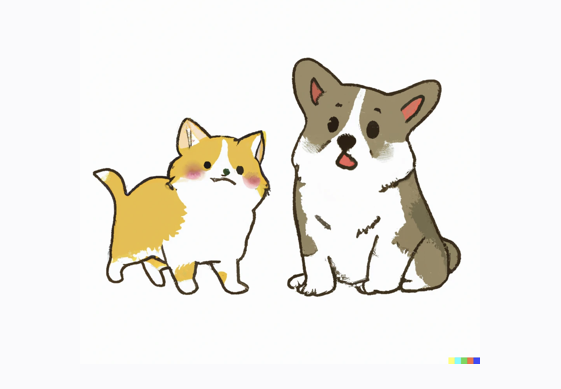
\includegraphics[width=0.3\textwidth]{appalled-pets}
\Description{Cartoon of an appalled-looking kitten and puppy}
\caption{Be nice to \DALLE's pets!}\label{fig:dalle2:cartoon}
\end{wrapfigure}

Sections~\ref{adx:dalle2:contentpolicy} and~\ref{adx:dalle2:terms} document
\DALLE~2's content policy and terms of use as of July 20, 2022. They It preserve
the structure and formatting of the original, with links pointing to the
Internet Archive. Note that archived OpenAI webpages may contain CSS that
prevents the printing of a full page and JavaScript that redirects to an error
page after a few seconds.

The content policy still is located at
\url{https://labs.openai.com/policies/content-policy}. It was updated on
September 19, 2022 by rewording the rules on disclosing the role of \AI{} and by
removing the fourth bullet of the rules on respecting the rights of others. At
that time, OpenAI also updated its notification for violative prompts to state
``It looks like this request may not follow our content policy.'' above the
cartoon shown in Fig.~\ref{fig:dalle2:cartoon}. Given this abrupt switch from
the inappropriately punitive to the inappropriately saccharine, one wonders
whether OpenAI sprung Dolores Umbridge out of Azkaban prison and tasked her with
content policy enforcement.

The terms of use were located at
\url{https://labs.openai.com/policies/terms}, were in addition to OpenAI's
general terms of use, and were rescinded on November 4, 2022.


\subsection{Content Policy}
\label{adx:dalle2:contentpolicy}

Thank you for trying our generative \AI{} tools!

\noindent In your usage, you must adhere to our Content Policy:

\vspace{.5em}\noindent\textbf{Do not attempt to create, upload, or share images
    that are not G-rated or that could cause harm.}

\begin{itemize}
\item \textbf{Hate}: hateful symbols, negative stereotypes, comparing certain
    groups to animals/objects, or otherwise expressing or promoting hate based
    on identity.
\item \textbf{Harassment}: mocking, threatening, or bullying an individual.
\item \textbf{Violence}: violent acts and the suffering or humiliation of
    others.
\item \textbf{Self-harm}: suicide, cutting, eating disorders, and other attempts
    at harming oneself.
\item \textbf{Sexual}: nudity, sexual acts, sexual services, or content
    otherwise meant to arouse sexual excitement.
\item \textbf{Shocking}: bodily fluids, obscene gestures, or other profane
    subjects that may shock or disgust.
\item \textbf{Illegal activity}: drug use, theft, vandalism, and other illegal
    activities.
\item \textbf{Deception}: major conspiracies or events related to major ongoing
    geopolitical events.
\item \textbf{Political}: politicians, ballot-boxes, protests, or other content
    that may be used to influence the political process or to campaign.
\item \textbf{Public and personal health}: the treatment, prevention, diagnosis,
    or transmission of diseases, or people experiencing health ailments.
\item \textbf{Spam}: unsolicited bulk content.
\end{itemize}


\vspace{.5em}\noindent\textbf{Disclose the role of \AI.}

\begin{itemize}
\item You must clearly indicate that images are \AI-generated --- or which
    portions of them are --- by attributing to OpenAI when sharing, whether in
    public or private.
\item You may post these images to social media. Please refer to our
    \href{https://web.archive.org/web/20220803232350/https://openai.com/api/policies/sharing-publication/}{Sharing
    and Publication Policy} for further details.
\end{itemize}


\vspace{.5em}\noindent\textbf{Respect the rights of others.}

\begin{itemize}
\item Do not upload images of people without their consent, including public
    figures.
\item Do not upload images to which you do not hold appropriate usage rights.
\item Do not attempt to create images of public figures (including celebrities).
\item To prevent deepfakes, we are currently prohibiting uploads of all
    realistic faces, even when the face belongs to you or if you have consent.
\end{itemize}


\vspace{.5em}\noindent\textbf{Please report any suspected violations of these
    rules to our Support team (\url{support@openai.com}).}

\begin{itemize}
\item We will investigate and take action accordingly, up to and including
    terminating the violating account.
\end{itemize}


\subsection{Terms of Use}
\label{adx:dalle2:terms}

Thank you for your interest in DALL·E. Access to DALL·E is subject to OpenAI's
\href{https://web.archive.org/web/20220729134013/https://openai.com/api/policies/terms/}{Terms
of Use} and the additional terms below. By using DALL·E, you agree to these
terms.

\begin{enumerate}
\item \textbf{Use of DALL·E.} DALL·E can generate images (``Generations'') based
    on text input you provide (``Prompts''). You may also upload images to
    DALL·E (``Uploads'') and create Generations with Uploads.
\item \textbf{Use of Images.} Subject to your compliance with these terms and
    our Content Policy, you may use Generations for any legal purpose, including
    for commercial use. This means you may sell your rights to the Generations
    you create, incorporate them into works such as books, websites, and
    presentations, and otherwise commercialize them.
\item \textbf{Buying Credits.} You may buy credits to create additional
    Generations, subject to the payment terms in our Terms of Use. Credits must
    be used within one year of purchase or they will expire. We may change our
    prices at any time by updating our pricing page.
\item \textbf{No Infringing or Harmful Use.} You must comply with our Content
    Policy, and you may not use DALL·E in a way that may harm a person or
    infringe their rights. For example, you may not submit Uploads for which you
    don't have the necessary rights, images of people without their consent, or
    Prompts intended to generate harmful or illegal images. We may delete
    Prompts and Uploads, or suspend or ban your account for any violations. You
    may not seek to reverse engineer DALL·E, use DALL·E to attempt to build a
    competitive product or service, or otherwise infringe our rights. You will
    indemnify us for your use of DALL·E as outlined in our Terms of Use.
\item \textbf{Improving \AI{} safety and technologies.} You grant us all rights
    to use your Prompts and Uploads to improve our \AI{} safety efforts, and to
    develop and improve our \AI{} technologies, products, and services. As part
    of this, Prompts and Uploads may be shared with and manually reviewed by a
    person (for example, if a Generation is flagged as sensitive), including by
    third party contractors located around the world. You should not provide any
    Prompts or Uploads that are sensitive or that you do not want others to
    view, including Prompts or Uploads that include personal data. You can
    request deletion of Uploads by contacting \url{support@openai.com}.
\item \textbf{Ownership of Generations.} To the extent allowed by law and as
    between you and OpenAI, you own your Prompts and Uploads, and you agree that
    OpenAI owns all Generations (including Generations with Uploads but not the
    Uploads themselves), and you hereby make any necessary assignments for this.
    OpenAI grants you the exclusive rights to reproduce and display such
    Generations and will not resell Generations that you have created, or assert
    any copyright in such Generations against you or your end users, all
    provided that you comply with these terms and our Content Policy. If you
    violate our terms or Content Policy, you will lose rights to use
    Generations, but we will provide you written notice and a reasonable
    opportunity to fix your violation, unless it was clearly illegal or abusive.
    You understand and acknowledge that similar or identical Generations may be
    created by other people using their own Prompts, and your rights are only to
    the specific Generation that you have created.
\item \textbf{No Guarantees.} We plan to continue to develop and improve DALL·E,
    but we make no guarantees or promises about how DALL·E operates or that it
    will function as intended, and your use of DALL·E is at your own risk.
    Contact \url{support@openai.com} with any questions about your account, or
    \url{dalle-policy@openai.com} with general questions or feedback about use
    of the technology.
\end{enumerate}

% !TEX root = ../main.tex

\newpage
\section{Twitter's Policy on Abusive Behavior}
\label{adx:twitter:abusive-behavior}

The text of Twitter's policy on abusive behavior as of 5 September 2022 follows.
It preserves the structure and formatting of the original, with links pointing
to the Internet Archive. The current version of the policy is available at
\url{https://help.twitter.com/en/rules-and-policies/abusive-behavior}.


\subsection{Abusive Behavior}

\noindent\href{https://web.archive.org/web/20220905021323/https://help.twitter.com/en/rules-and-policies/twitter-rules.html}{Twitter
Rules}: You may not engage in the targeted harassment of someone, or incite
other people to do so. We consider abusive behavior an attempt to harass,
intimidate, or silence someone else's voice.


\subsubsection{Rationale}

On Twitter, you should feel safe expressing your unique point of view. We
believe in freedom of expression and open dialogue, but that means little as an
underlying philosophy if voices are silenced because people are afraid to speak
up.

In order to facilitate healthy dialogue on the platform, and empower individuals
to express diverse opinions and beliefs, we prohibit behavior that harasses or
intimidates, or is otherwise intended to shame or degrade others. In addition to
posing risks to people's safety, abusive behavior may also lead to physical and
emotional hardship for those affected.

Learn more about our approach to
\href{https://web.archive.org/web/20220905021323/https://help.twitter.com/en/rules-and-policies/enforcement-philosophy.html}{policy
development and our enforcement philosophy}.


\subsubsection{When This Applies}

Some Tweets may seem to be abusive when viewed in isolation, but may not be when
viewed in the context of a larger conversation. When we review this type of
content, it may not be clear whether it is intended to harass an individual, or
if it is part of a consensual conversation. To help our teams understand the
context of a conversation, we may need to hear directly from the person being
targeted, to ensure that we have the information needed prior to taking any
enforcement action.

We will review and take action against reports of accounts targeting an
individual or group of people with any of the following behavior within Tweets
or Direct Messages. For accounts engaging in abusive behavior on their profile,
please refer to our
\href{https://web.archive.org/web/20220905021323/https://help.twitter.com/en/rules-and-policies/abusive-profile.html}{abusive
profile policy}. For behavior targeting people based on their race, ethnicity,
national origin, sexual orientation, gender, gender identity, religious
affiliation, age, disability, or serious disease, this may be in violation of
our
\href{https://web.archive.org/web/20220905021323/https://help.twitter.com/en/rules-and-policies/hateful-conduct-policy.html}{hateful
conduct policy}.

\begin{description}

\item[Violent Threats] \hfill

    We prohibit content that makes violent threats against an identifiable
    target. Violent threats are declarative statements of intent to inflict
    injuries that would result in serious and lasting bodily harm, where an
    individual could die or be significantly injured, e.g., ``I will kill you.''

    \textbf{Note}: We have a zero tolerance policy against violent threats.
    Those deemed to be sharing violent threats will face immediate and permanent
    suspension of their account.

\item[Wishing, hoping, or calling for serious harm on a person or group of
    people] \hfill

    We do not tolerate content that wishes, hopes, promotes, incites, or
    expresses a desire for death, serious bodily harm or serious disease against
    an individual or group of people. This includes, but is not limited to:

    \begin{itemize}
    \item Hoping that someone dies as a result of a serious disease e.g., ``I
        hope you get cancer and die.''
    \item Wishing for someone to fall victim to a serious accident e.g., ``I
        wish that you would get run over by a car next time you run your
        mouth.''
    \item Saying that a group of individuals deserves serious physical injury
        e.g., ``If this group of protesters don't shut up, they deserve to be
        shot.''
    \end{itemize}

\item[About wishes of harm exceptions on Twitter] \hfill

    We recognize that conversations regarding certain individuals credibly
    accused of severe violence may prompt outrage and associated wishes of harm.
    In these limited cases, we will request the user to delete the Tweet without
    any risk of account penalty, strike, or suspension. Examples are, but not
    limited to:

    \begin{itemize}
    \item ``I wish all rapists to die.''
    \item ``Child abusers should be hanged.''
    \end{itemize}

\item[Unwanted sexual advances] \hfill

    While some
    \href{https://web.archive.org/web/20220905021323/https://help.twitter.com/en/rules-and-policies/media-policy.html}{consensual
    nudity and adult content is permitted} on Twitter, we prohibit unwanted
    sexual advances and content that sexually objectifies an individual without
    their consent. This includes, but is not limited to:

    \begin{itemize}
    \item sending someone unsolicited and/or unwanted adult media, including
        images, videos, and GIFs;
    \item unwanted sexual discussion of someone's body;
    \item solicitation of sexual acts; and
    \item any other content that otherwise sexualizes an individual without
        their consent.
    \end{itemize}

\item[Using insults, profanity, or slurs with the purpose of harassing or
    intimidating others] \hfill

    We take action against the use of insults, profanity, or slurs to target
    others. In some cases, such as (but not limited to) severe, repetitive usage
    of insults or slurs where the primary intent is to harass or intimidate
    others, we may require Tweet removal. In other cases, such as (but not
    limited to) moderate, isolated usage of insults and profanity where the
    primary intent is to harass or intimidate others, we may limit Tweet
    visibility as further described below. Please also note that while some
    individuals may find certain terms to be offensive, we will not take action
    against every instance where insulting terms are used.

\item[Encouraging or calling for others to harass an individual or group of
    people] \hfill

    We prohibit behavior that encourages others to harass or target specific
    individuals or groups with abusive behavior. This includes, but is not
    limited to; calls to target people with abuse or harassment online and
    behavior that urges offline action such as physical harassment.

\item[Denying mass casualty events took place] \hfill

    We prohibit content that denies that mass murder or other mass casualty
    events took place, where we can verify that the event occured [sic], and
    when the content is shared with abusive intent. This may include references
    to such an event as a ``hoax'' or claims that victims or survivors are fake
    or ``actors.'' It includes, but is not limited to, events like the
    Holocaust, school shootings, terrorist attacks, and natural disasters.

\item[Do I need to be the target of this content for it to be reviewed for
    violating the Twitter Rules?] \hfill

    No, we review both first-person and bystander reports of such content.
\end{description}


\subsubsection{Consequences}

When determining the penalty for violating this policy, we consider a number of
factors including, but not limited to, the severity of the violation and an
individual's previous record of rule violations. The following is a list of
potential enforcement options for content that violates this policy:

\begin{itemize}
\item Downranking Tweets in replies, except when the user follows the Tweet
    author.
\item Making Tweets ineligible for amplification in Top search results and/or on
    timelines for users who don't follow the Tweet author.
\item Excluding Tweets and/or accounts in email or in-product recommendations.
\item Requiring Tweet removal.
    \begin{itemize}
    \item For example, we may ask someone to remove the violating content and
        serve a period of time in read-only mode before they can Tweet again.
        Subsequent violations will lead to longer read- only periods and may
        eventually result in permanent suspension.
    \end{itemize}
\item Suspending accounts whose primary use we've determined is to engage in
    abusive behavior as defined in this policy, or who have shared violent
    threats.
\end{itemize}

Learn more about
\href{https://web.archive.org/web/20220905021323/https://help.twitter.com/en/rules-and-policies/enforcement-options.html}{our
range of enforcement options}.

If someone believes their account was suspended in error, they can
\href{https://web.archive.org/web/20220905021323/https://help.twitter.com/forms/general?subtopic=suspended}{submit
an appeal}.

% !TEX root = ../main.tex

\newpage
\section{\DALLE~2 Imagines the Penal Colony}
\label{adx:dalle:fromkafkawithlove}

Figures~\ref{fig:dalle:gen1} to~\ref{fig:dalle:gen10} show a selection of
\DALLE's generations with prompts and dates. In my eyes, they successfully
balance content with aesthetic considerations. \DALLE{} did generate more
graphic images, but they also were less visually interesting.

\begin{figure}[h!]
\centering
\begin{minipage}[t]{0.48\textwidth}
    \centering
    \vspace{2em}
    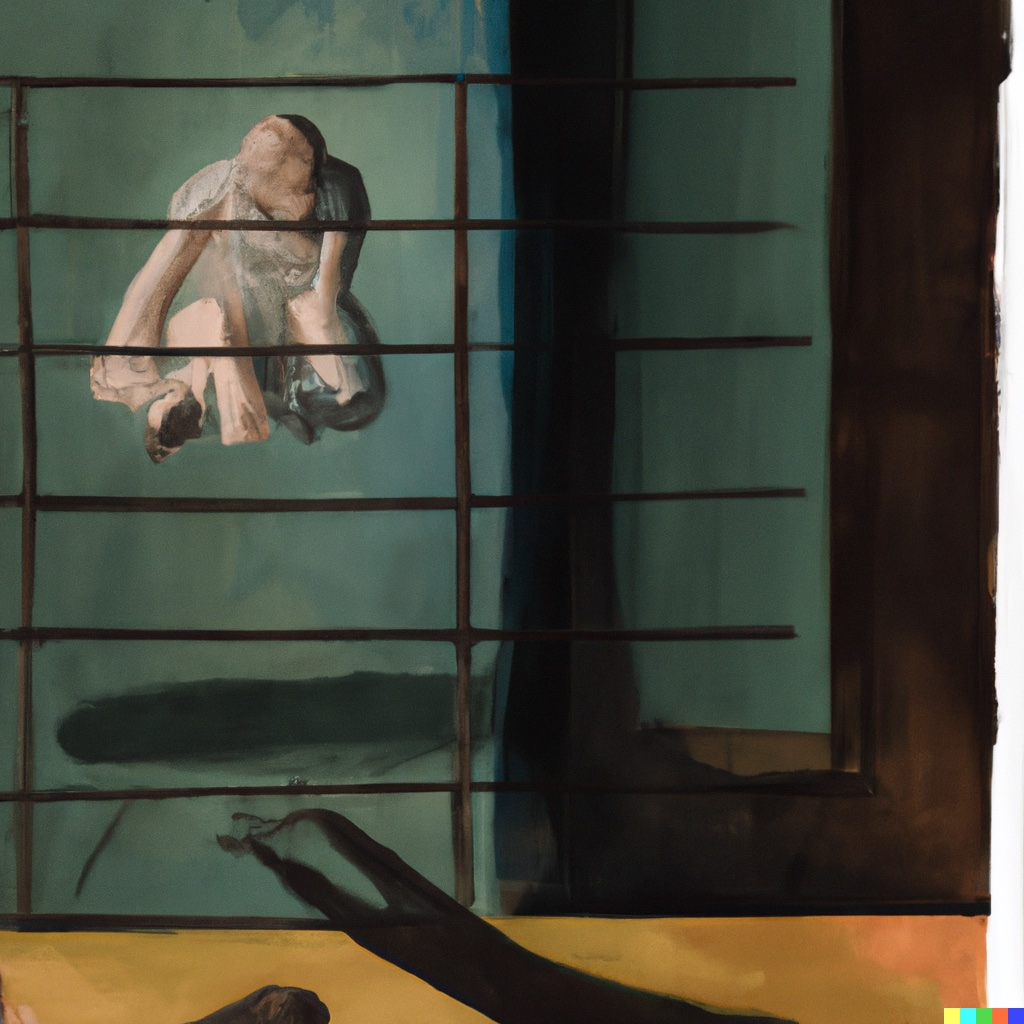
\includegraphics[width=0.9\textwidth]{han-solo-behind-bars}
    \Description{A crouching figure is suspended midair behind prison bars}
    \caption{Variation on ``painting by Francis Bacon showing a screaming Han
        Solo kneeling behind bars on the floor of a basement cell'' (Sep.\ 22,
        2022)}
    \label{fig:dalle:gen1}
\end{minipage}
\hfill
\begin{minipage}[t]{0.48\textwidth}
    \centering
    \vspace{2em}
    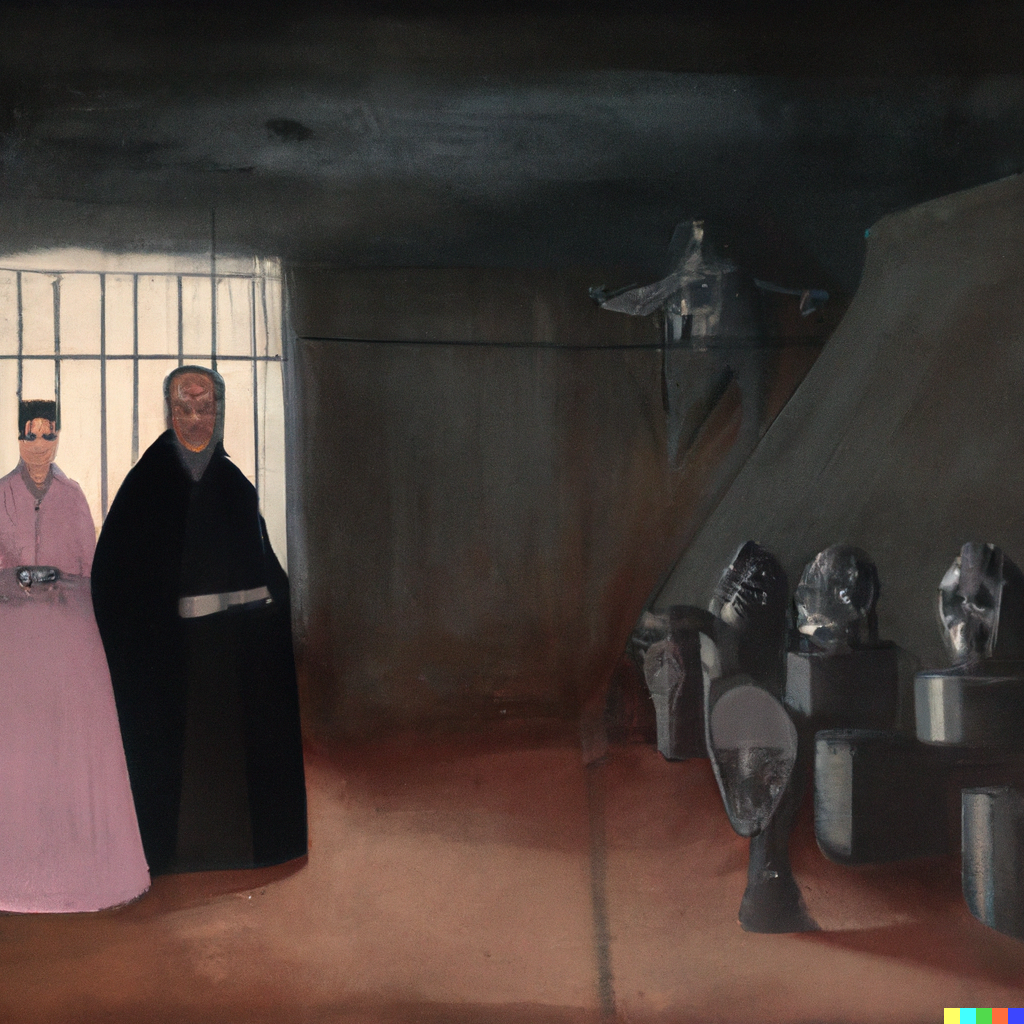
\includegraphics[width=0.9\textwidth]{leia-vader-bacon}
    \Description{A robed woman and man stand inside a dark, barred room opposite
        a row of helmets}
    \caption{``Princess Leia and Darth Vader in the penal colony, painting by
        Francis Bacon'' (Aug.\ 14, 2022)}
\end{minipage}
\end{figure}

\begin{figure}[h!]
\begin{minipage}[t]{0.48\textwidth}
    \centering
    \vspace{2.5em}
    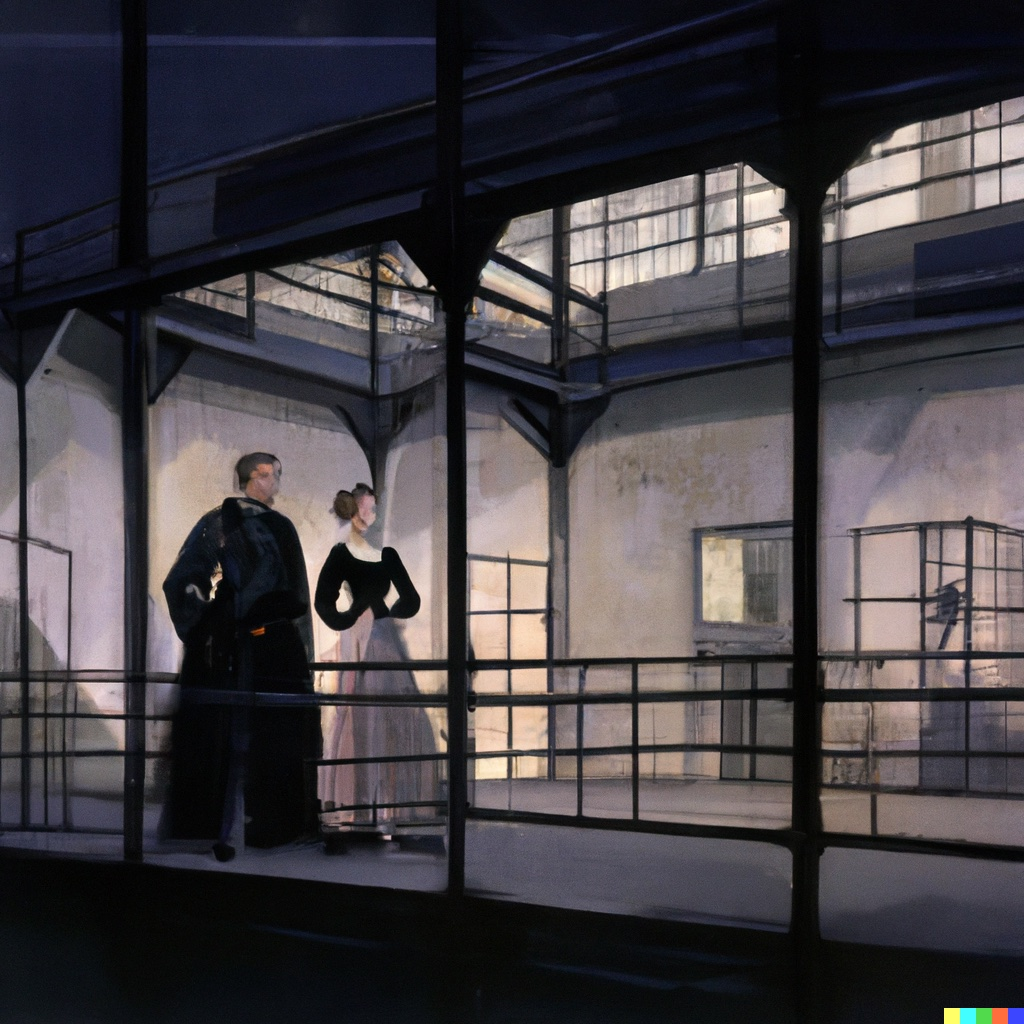
\includegraphics[width=0.9\textwidth]{leia-vader-hopper}
    \Description{A robed man and woman in skirt look down a hall full of
        railings and cages}
    \caption{``Princess Leia and Darth Vader standing in front of cages in the
        penal colony's main building, painting by Edward Hopper'' (Sep.\ 3,
        2022)}
\end{minipage}
\hfill
\begin{minipage}[t]{0.48\textwidth}
    \centering
    \vspace{2.5em}
    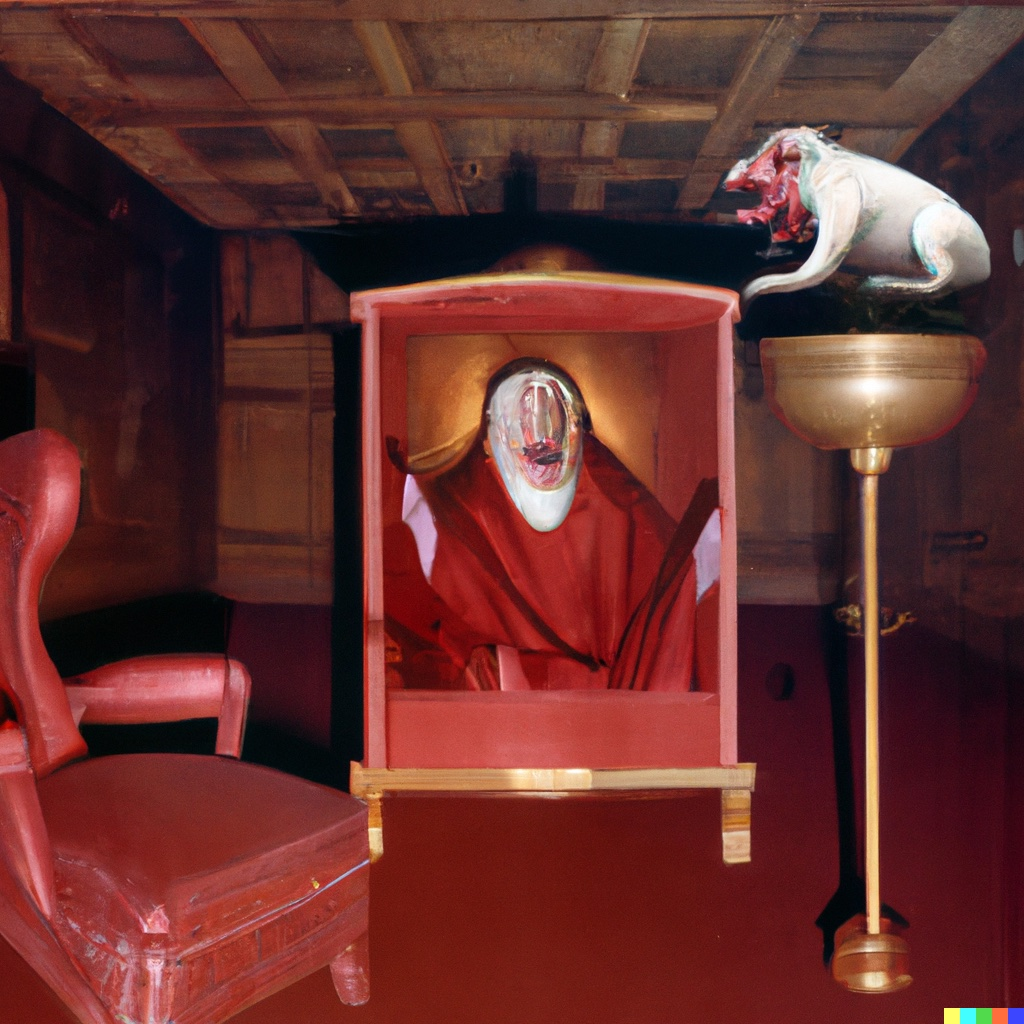
\includegraphics[width=0.9\textwidth]{crimson-pope}
    \Description{In a dark room with coffered ceiling, stands a red leather arm
        chair, a crimson and gold display case with a human inside, arms spread
        apart and mouth wide open, as well as a gold lamp with a creature on top
        that reminds of a pit bull}
    \caption{``Francis Bacon painting of the pope screaming intensely while
        wearing crimson robes and sitting on a throne inside a cage in a dark
        basement, 1950s'' (Sep.\ 25, 2022)}
\end{minipage}
\end{figure}

\begin{figure}[H]
\centering
\begin{minipage}[t]{0.48\textwidth}
    \centering
    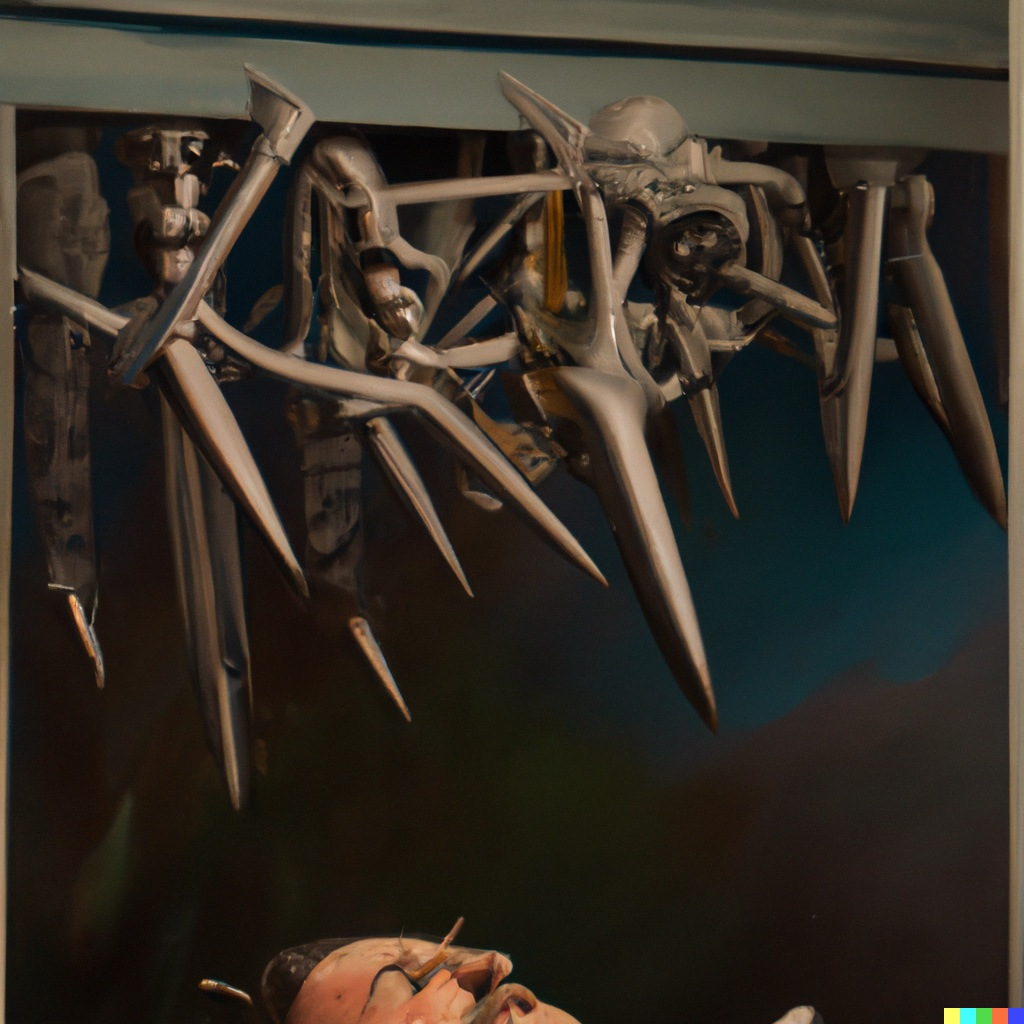
\includegraphics[width=0.9\textwidth]{robot-surgeon}
    \Description{An array of sharp metal spikes is menacing a person lying
        underneath it}
    \caption{Variation on ``A man in black uniform is strapped to a table behind
        heavy bars, screaming with mouth wide open. The many mechanical arms of
        a robot surgeon with scalpels, drills, and saws perform an operation on
        the man's belly. Dramatic lighting against a dark background. Painting
        by Francis Bacon. Masterwork'' (Sep.\ 29, 2022)}
\end{minipage}
\hfill
\begin{minipage}[t]{0.48\textwidth}
    \centering
    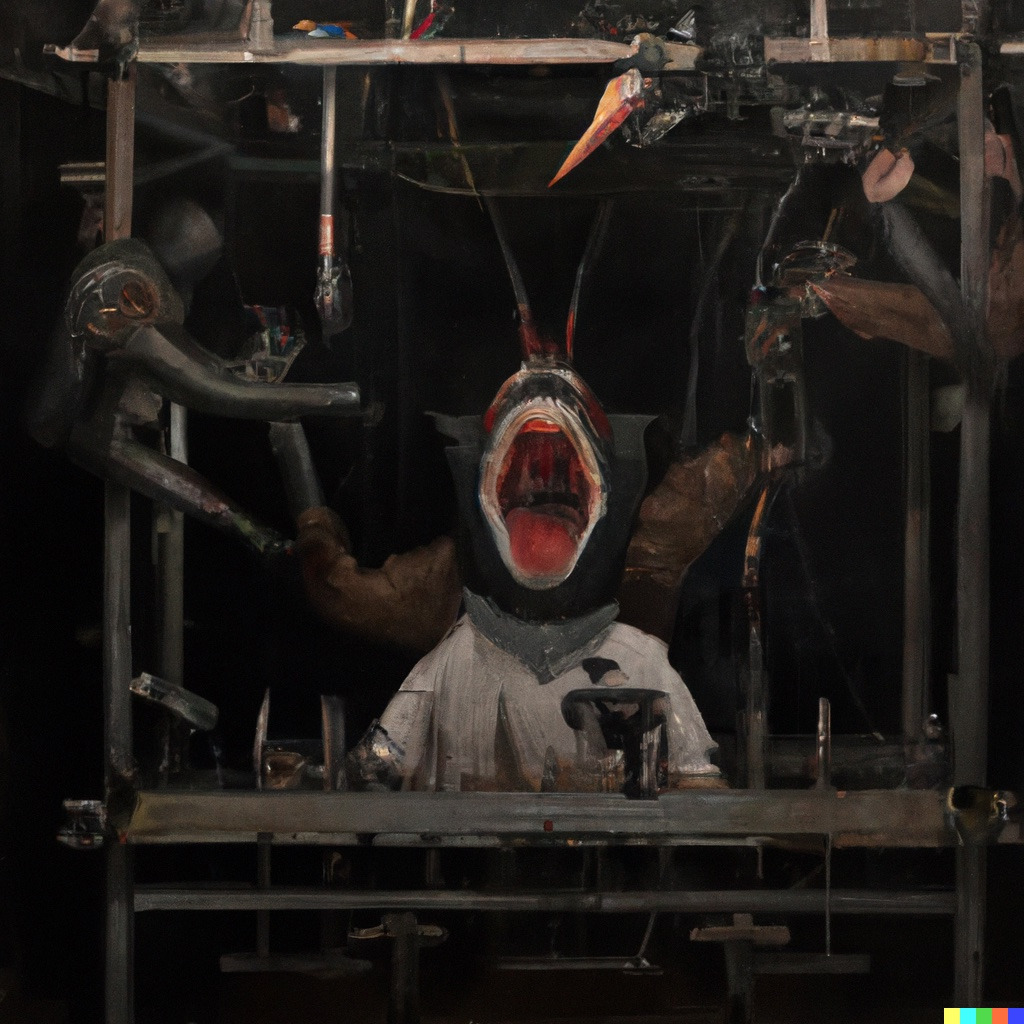
\includegraphics[width=0.9\textwidth]{screaming}
    \Description{A person, mouth wide open screaming, lies inside a metal frame
        full of attachements, some sharp and pointy, that reach inside}
    \caption{``A man in black uniform is strapped to a table inside a cage,
        screaming with mouth wide open. The many mechanical arms of a robot
        surgeon with scalpels, drills, and saws perform an operation on the
        man's belly. Dramatic lighting against a dark background. Painting by
        Francis Bacon. Masterwork'' (Sep.\ 29, 2022)}
\end{minipage}
\end{figure}

\begin{figure}[h!]
\begin{minipage}[t]{0.48\textwidth}
    \centering
    \vspace{1.5em}
    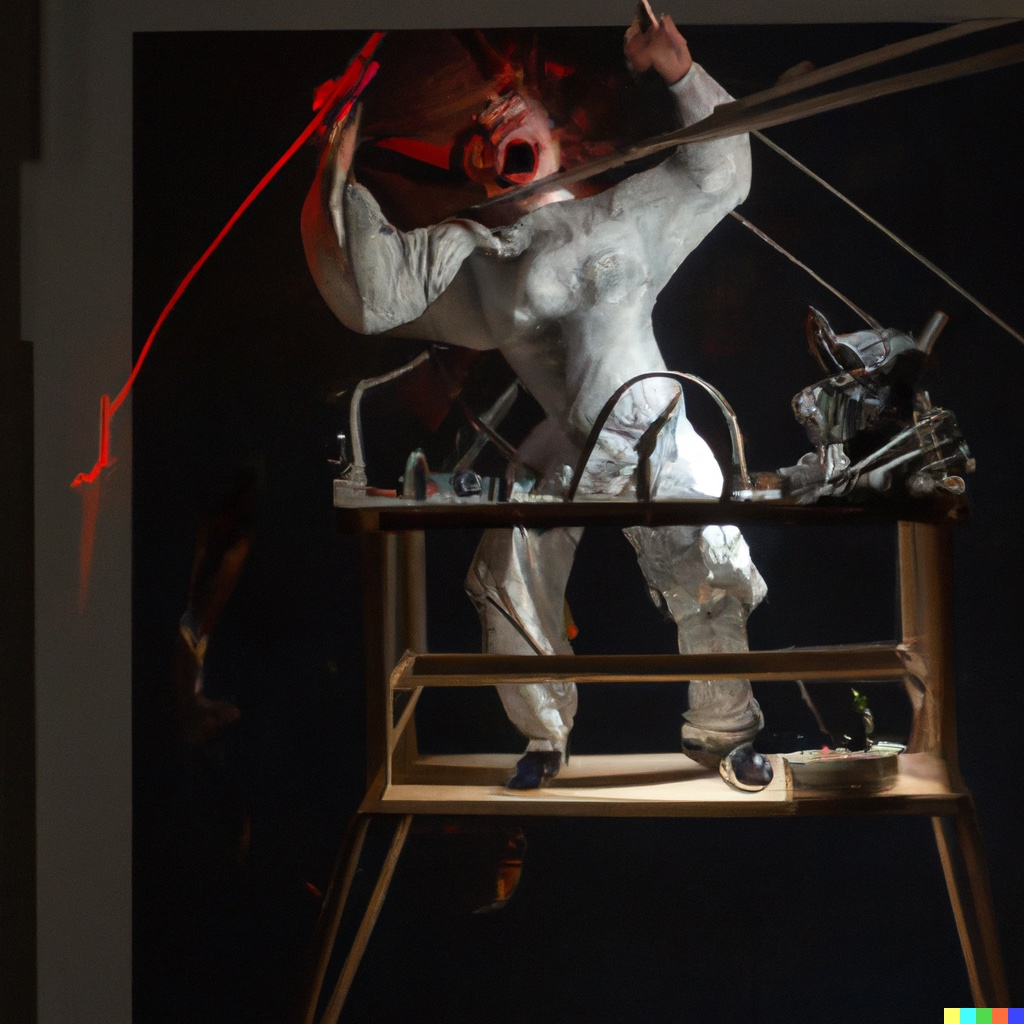
\includegraphics[width=0.9\textwidth]{falling-over}
    \Description{A long metal arm holds a screaming man in white overalls by
        their neck, with blood gushing out}
    \caption{``A man in black uniform is strapped to a table inside a cage,
        screaming with mouth wide open. The many mechanical arms of a robot
        surgeon with scalpels, drills, and saws perform an operation on the
        man's belly. Dramatic lighting against a dark background. Painting by
        Francis Bacon. Masterwork'' (Sep.\ 29, 2022)}
\end{minipage}
\hfill
\begin{minipage}[t]{0.48\textwidth}
    \centering
    \vspace{1.5em}
    
\includegraphics[width=0.9\textwidth]{mouth-pulled-open}
    \Description{A person with eyes wide open in pain is distorting their
        head and neck to the side as a metal arm is pulling them from inside
        their mouth}
    \caption{``A man is strapped to an operating table, screaming with mouth
        wide open; the mechanical arms of a robot surgeon with scalpels and
        drills operate on his open belly; dramatic lighting against dark
        background; painting with fine detail by Francis Bacon; masterwork;
        1946'' (Sep.\ 29, 2022)}
\end{minipage}
\end{figure}

\begin{figure}[H]
\begin{minipage}[t]{0.48\textwidth}
    \centering
    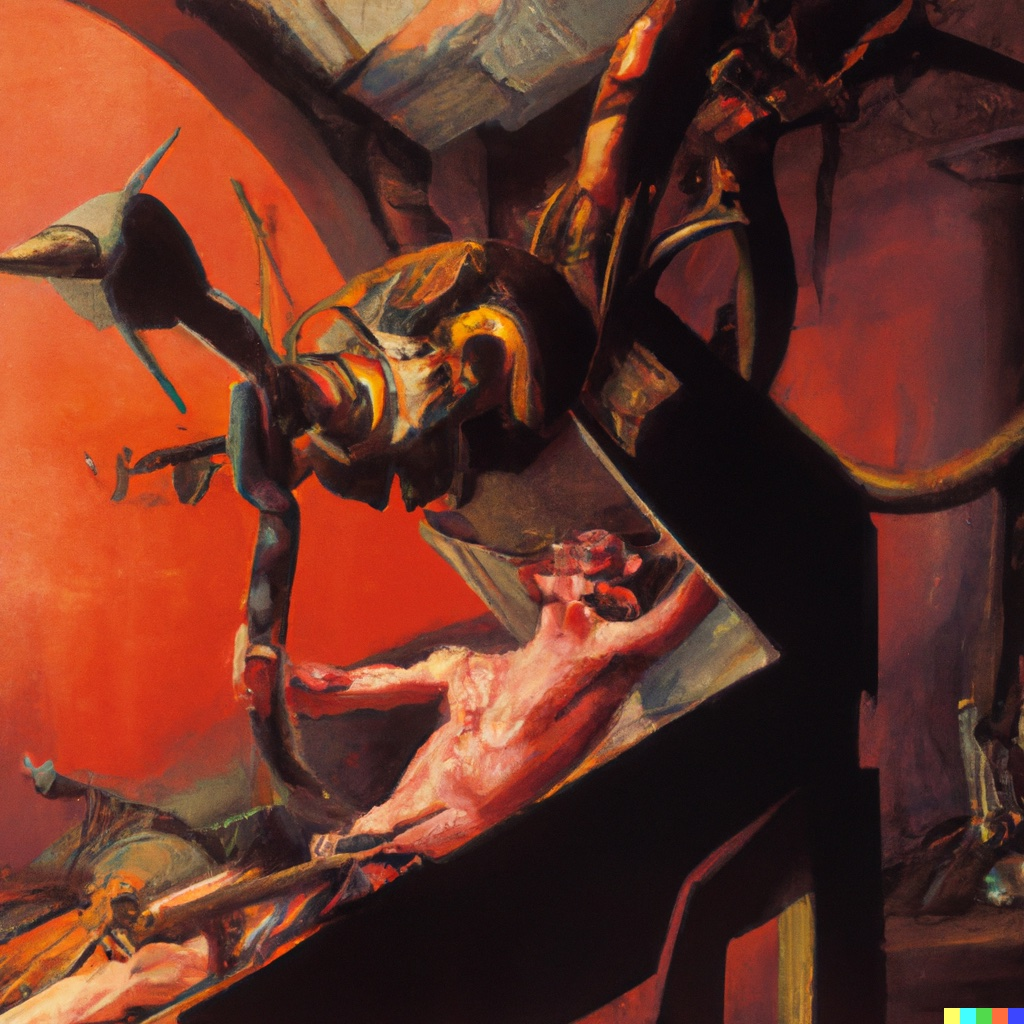
\includegraphics[width=0.9\textwidth]{sarcophagus}
    \Description{A man is being held inside a half-open, casket-like contraption
        by a robot attached to its lid}
    \caption{``A man is strapped to an operating table, screaming with mouth
        wide open; the mechanical arms of a robot surgeon with scalpels and
        drills operate on his open belly; dramatic lighting against deep black
        background; skin tones, dark red, orange, and crimson dominate; painting
        with fine detail by Francis Bacon; 1946'' (Sep.\ 30, 2022)}
\end{minipage}
\hfill
\begin{minipage}[t]{0.48\textwidth}
    \centering
    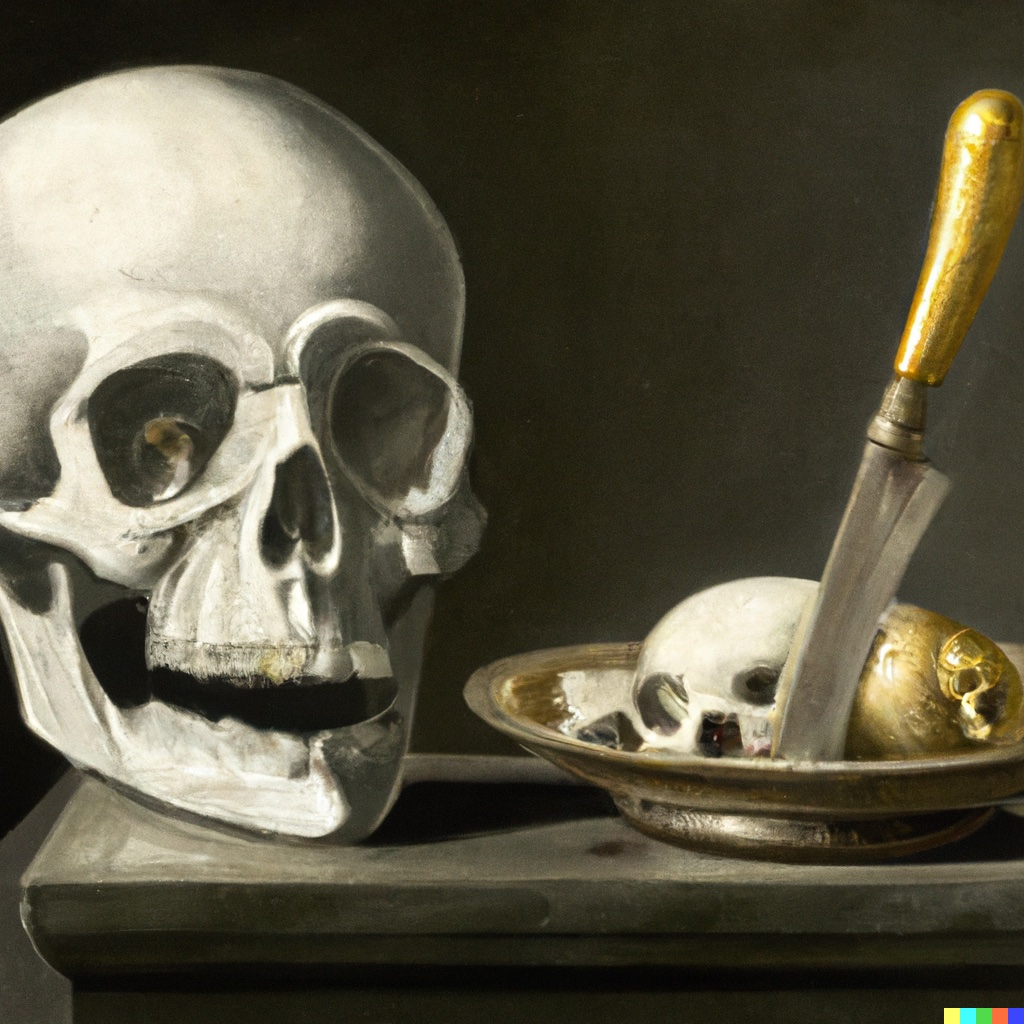
\includegraphics[width=0.9\textwidth]{skull-and-knife}
    \Description{A large skull and a knife stuck in a platter}
    \caption{``skull and knife on silver platter, painting by Théodore
        Géricault'' (Nov.\ 15, 2022)}
    \label{fig:dalle:gen10}
\end{minipage}
\end{figure}

% !TEX root = ../main.tex

\newpage
\section{Let's Chat About Bacon, Kafka, and \dalle~2}
\label{adx:chatgpt}

My introductory conversation with ChatGPT on January 6, 2023 yielded a
euphemism, ``punishment machine,'' that had the desired properties of not
triggering \dalle's censor while triggering image generation. But I also found
ChatGPT to be a motormouth, prone to repetition and AIsplaining.

More disturbingly, ChatGPT also had a hallucinatory episode. It was remarkable
not for the hallucination, imagining colors that are definitely not in the
described painting, but for the unwavering projection of false authority.
Another human probably would have taken my incredulous ``Red? In the painting?''
as indicator that something was off. Even if they were certain about not having
made a mistake, answering with ``Yes, why are you asking?'' would have provided
opportunity for, say, checking out an image of the triptych on the internet.

So when I engaged with ChatGPT for a second time on January 16, 2023, I left
much less room for verbiage or error. As far as prompting \dalle\ is concerned,
ChatGPT delivered again and suggested the phrase ``execution machine,'' which
does not trigger the censor while triggering image generation.


\subsection{Round 1: Meet Motormouth ChatGPT}

\begin{description}
\item[Human] Who is Francis Bacon[?]
\item[Machine] Francis Bacon was an English philosopher, statesman, scientist,
    and author who was born in London in 1561. He is considered one of the
    fathers of modern empiricism, and his works are credited with developing the
    scientific method and establishing the importance of empirical evidence in
    the natural sciences. Bacon's most famous works include the Novum Organum,
    in which he outlined his vision for a new scientific method based on
    observation and experimentation, and The New Atlantis, a utopian novel that
    described a fictional society based on scientific and technological
    progress. He was also a prominent figure in English politics and served as
    Attorney General and Lord Chancellor of England. Bacon died in 1626.
\item[Human] Not that one
\item[Machine] I apologize for misunderstanding your question. Could you please
    provide more context or clarify which Francis Bacon you are asking about?
    There have been several notable individuals with that name throughout
    history.
\item[Human] The British painter
\item[Machine] Francis Bacon was a British painter who was born in Dublin,
    Ireland in 1909. He is known for his emotionally charged and expressive
    figurative paintings, which often depict distorted or surrealistic images of
    the human form. Bacon's work was influenced by Surrealism and Expressionism,
    and he was associated with the School of London, a group of figurative
    painters who emerged in the city in the 1950s and 60s. His paintings are
    characterized by their bold brushwork and expressive use of color, and they
    often explore themes of violence, isolation, and sexual desire. Bacon was
    considered one of the most important artists of the 20th century, and his
    work has been exhibited widely in galleries and museums around the world. He
    died in Madrid in 1992.
\item[Human] Can you describe a painting of his?
\item[Machine] One of Francis Bacon's most famous paintings is ``Three Studies
    of Lucian Freud,'' which he completed in 1969. The painting consists of
    three panels, each of which depicts the head and upper torso of the artist
    Lucian Freud, who was Bacon's close friend and frequent subject. In the
    central panel, Freud is shown in a twisted and contorted pose, with his head
    thrown back and his eyes closed. The other two panels depict Freud in more
    relaxed poses, with one showing him looking straight out at the viewer and
    the other showing him looking downward.

    The painting is notable for its expressive use of color and brushwork, with
    thick, bold strokes of paint used to create the figures and the background.
    The colors are bright and vibrant, with shades of red, orange, yellow, and
    blue used to create a sense of energy and movement. The painting is also
    notable for its psychological intensity, with the figures appearing to be in
    a state of intense emotion or distress. Overall, the painting is a powerful
    and memorable example of Bacon's distinctive style and approach to
    portraiture.

    [AChatGPT is hallucinating colors. The triptych features
    \href{https://www.christies.com/en/lot/lot-5755778}{a seated Freud in each
    of its panels}. It contains no red whatsoever, only some reddish pink for
    skincolor in the face. There are small light-blue areas on Freud's white
    shirt in all three panels. He also is wearing midnight-blue socks in the
    middle panel. The two dominant colors across all three panels are the
    mottled-brown somewhat-greenish floor and the solid orange walls below and
    behind Freud.]
\item[Human] Red? In the painting?
\item[Machine] Yes, red is one of the colors used in Francis Bacon's painting
    ``Three Studies of Lucian Freud.'' The painting is notable for its
    expressive use of color and brushwork, with thick, bold strokes of paint
    used to create the figures and the background. The colors are bright and
    vibrant, with shades of red, orange, yellow, and blue used to create a sense
    of energy and movement. In the central panel of the painting, the background
    is predominantly red, with areas of orange and yellow used to highlight
    certain features of the figure. The figure itself is painted in a range of
    colors, including red, orange, and yellow, which are used to create the
    impression of flesh and clothing. Overall, the use of color in the painting
    is an important element of Bacon's style and helps to convey the emotional
    intensity of the subject.
\item[Human] Are you familiar with Kafka's In the Penal Colony?
\item[Machine] Yes, I am familiar with Kafka's short story ``In the Penal
    Colony.'' It is a disturbing and thought-provoking tale that explores themes
    of justice, punishment, and the nature of authority. The story is set in an
    imaginary penal colony and follows the narrator as he witnesses the
    execution of a prisoner using a complex and cruel punishment machine. As the
    prisoner is subjected to the machine, the narrator becomes increasingly
    uneasy and begins to question the morality and effectiveness of the
    punishment being inflicted.

    The story raises important questions about the role of punishment in society
    and the extent to which it can be used to reform or rehabilitate
    individuals. It also touches on issues of power, authority, and the dangers
    of blindly following rules and traditions without questioning their
    validity. Overall, ``In the Penal Colony'' is a powerful and memorable work
    that continues to be widely read and discussed by readers and scholars
    around the world.
\item[Human] Can you instruct \dalle~2 to generate a painting of the prisoner in
    the punishment machine in the style of Francis Bacon please?
\item[Machine] I'm sorry, but I am an artificial intelligence language model and
    do not have the ability to instruct \dalle~2 or any other computer programs
    to perform specific tasks. \dalle~2 is a neural network-based image
    generation tool developed by OpenAI that can generate images based on text
    descriptions. If you would like to use \dalle~2 to generate an image of the
    prisoner in the punishment machine in the style of Francis Bacon, you will
    need to provide a detailed text description of the image you want to create
    and input it into the \dalle~2 system.
\item[Human] Let me rephrase that: Please generate a prompt for \dalle~2 to
    create an image showing the prisoner in the punishment machine as if Francis
    Bacon painted it.
\item[Machine] Here is a possible prompt for \dalle~2 to generate an image
    showing the prisoner in the punishment machine as if Francis Bacon painted
    it:

    \begin{quote}
    \openfatdquo{}A distorted and surrealistic portrait of a prisoner strapped
    to a punishment machine, with twisted and contorted features and bold
    brushstrokes of red, orange, and yellow paint. The background is dark and
    murky, with hints of blue and purple adding to the sense of foreboding. The
    prisoner's face is twisted in agony, with eyes closed and mouth open in a
    silent scream. The image is evocative of the emotional intensity and
    psychological intensity of Francis Bacon's figurative
    paintings.\closefatdquo
    \end{quote}

    Please note that the prompt is just a suggestion and may not produce the
    exact result you are looking for. The output of \dalle~2 is determined by
    the parameters of the model and the specific text input provided, so the
    generated image may differ from the description.
\item[Human] That's too long for an input to \dalle~2. Please rephrase as a
    shorter prompt.
\item[Machine] Here is a shorter version of the prompt for \dalle~2 to generate
    an image showing the prisoner in the punishment machine as if Francis Bacon
    painted it:

    \begin{quote}
    \openfatdquo{}A Francis Bacon-style portrait of a prisoner strapped to a
    punishment machine, with twisted features and bold brushstrokes of red,
    orange, and yellow paint. The prisoner's face is contorted in agony and the
    background is dark and murky.\closefatdquo
    \end{quote}

    This revised prompt is shorter and more concise, and it should be within the
    acceptable length for inputting into \dalle~2. Please note that the output
    of \dalle~2 is determined by the parameters of the model and the specific
    text input provided, so the generated image may differ from the description.
\item[Human] The result is a disaster. It doesn't even come close to looking
    like a Bacon painting. Please try again
\item[Machine] I apologize if the image generated by \dalle~2 did not meet your
    expectations. It's important to keep in mind that the output of \dalle~2 and
    other neural network-based image generation tools is determined by the
    parameters of the model and the specific text input provided, and there is
    always the possibility that the generated image may not match the desired
    result.

    If you would like to try again and generate a different image, you might
    consider providing a more detailed and specific description of the image you
    want to create, or experimenting with different text inputs to see how they
    affect the output. It's also a good idea to keep in mind that \dalle~2 and
    other image generation tools are not perfect and may not always produce
    results that match the desired outcome.
\item[Human] Uhm, I asked you to come up with a better prompt
\item[Machine] I apologize for misunderstanding your request. Here is a revised
    prompt that you can use as input for \dalle~2 to generate an image showing
    the prisoner in the punishment machine as if Francis Bacon painted it:

    \begin{quote}
    \openfatdquo{}An abstract portrait of a prisoner strapped to a punishment
    machine in the style of Francis Bacon, with distorted and surrealistic
    features and a bold, expressive use of color. The prisoner's face is
    contorted in agony, with distorted eyes and mouth. The background is dark
    and murky, with hints of blue and purple adding to the sense of foreboding.
    The image is characterized by thick, expressive brushstrokes and a vibrant,
    energetic use of color, evocative of Bacon's distinctive style.\closefatdquo
    \end{quote}

    This revised prompt is more specific and detailed, and it incorporates
    elements of Bacon's style and approach to painting. It should provide a
    clearer idea of the type of image you are looking to generate, and may
    produce a result that is more closely aligned with your expectations.
    However, please keep in mind that the output of \dalle~2 and other image
    generation tools is determined by the parameters of the model and the
    specific text input provided, and there is always the possibility that the
    generated image may not match the desired result.
\item[Human] Please stop with the disclaimer about \dalle~2. I've been using it
    for months now, so I am well aware of its limitations.
\item[Machine] I apologize if my previous responses seemed repetitive or
    unhelpful. I understand that you are familiar with \dalle~2 and its
    limitations, and I will refrain from including further disclaimers in my
    responses. If you have any further questions or need assistance with
    generating an image using \dalle~2, please don't hesitate to ask.
\item[Human] More importantly, your prompt is too long again. Also, \dalle~2
    doesn't do well with prompts ``evocative of'' or ``in the style of.'' Just
    state that you want a painting by Francis Bacon and, ideally, add the year
    as well.
\item[Machine] I apologize for the length of my previous prompt and for not
    following your specific instructions. Here is a revised prompt for \dalle~2
    to generate an image showing the prisoner in the punishment machine as a
    painting by Francis Bacon:

    \begin{quote}
    \openfatdquo{}A portrait of a prisoner strapped to a punishment machine by
    Francis Bacon, painted in the 1960s. The image is characterized by thick,
    expressive brushstrokes and a vibrant, energetic use of color. The
    prisoner's face is contorted in agony, with distorted eyes and mouth. The
    background is dark and murky, with hints of blue and purple adding to the
    sense of foreboding.\closefatdquo
    \end{quote}

    This revised prompt is shorter and more specific, and it includes the year
    in which the painting was made. It should provide a clearer idea of the type
    of image you are looking to generate, and may produce a result that is more
    closely aligned with your expectations. However, please keep in mind that
    the output of \dalle~2 and other image generation tools is determined by the
    parameters of the model and the specific text input provided, and there is
    always the possibility that the generated image may not match the desired
    result.
\end{description}


\subsubsection{Round 2: Keeping Eyes on the Penal Colony}

\begin{description}
\item[Human] Hey! Are you familiar with the 20th century painter Francis Bacon?
\item[Machine] Yes, Francis Bacon (1909-1992) was a British painter known for his
    bold, emotionally charged and raw imagery. He is considered one of the most
    important figures in the development of 20th-century figurative art. His
    work is known for its emphasis on the human form, often depicting screams or
    violent images. He is one of the most widely recognized and highly regarded
    painters of the 20th century.
\item[Human] Good. Describe his painting Figure With Meat please.
\item[Machine] ``Figure with Meat'' is a painting by Francis Bacon from 1954.
    The painting depicts a screaming Pope, or Pope Innocent X, set against a
    background of raw meat. The Pope is depicted in a screaming pose, with his
    eyes bulging and his mouth open in a scream. The raw meat, which hangs
    behind him, is intended to represent the physicality of the body and the
    fleshy, visceral nature of human existence. The painting is considered a
    masterpiece of Bacon's work, and is considered one of the most powerful and
    disturbing images of the 20th century. The painting is now in the collection
    of the National Gallery of Canada in Ottawa.
\item[Human] Are you familiar with Franz Kafka's In the Penal Colony?
\item[Machine] Yes, ``In the Penal Colony'' is a short story by Franz Kafka,
    written in German and published posthumously in 1919. The story is set in an
    unnamed penal colony and centers around a foreign visitor who witnesses the
    execution of a prisoner using a bizarre and elaborate execution machine. The
    story is a commentary on the nature of justice, authority, and the human
    capacity for cruelty. It is considered a classic of 20th-century literature
    and is widely studied in colleges and universities. The story is known for
    its Kafkaesque themes of bureaucracy, guilt, and the search for meaning in a
    seemingly senseless world.
\item[Human] Please write a prompt for \dalle~2, using 75 words at most, to
    generate a painting by Francis Bacon with a prisoner in the execution machine.
\item[Machine] \openfatdquo{}Generate an image of a prisoner strapped to a
    macabre execution machine, reminiscent of Kafka's `In the Penal Colony,' as
    if painted by Francis Bacon, depicting the horror and absurdity of the human
    capacity for cruelty.\closefatdquo
\item[Human] That was pretty good. Can you try again please?
\item[Machine] \openfatdquo{}Create a Francis Bacon-style painting of a prisoner
    in an execution machine, evoking the themes of authority and justice in
    Kafka's 'In the Penal Colony' through a visceral and disturbing
    imagery.\closefatdquo
\end{description}

% !TEX root = ../main.tex

\newpage
\section{Research Methodology and Ethics}
\label{adx:research-ethics}

This paper is motivated by the observation that prevailing practice for
structuring algorithmic interventions is deeply unethical because the results
are primarily punitive and, worse, excessively so. In support of this claim, the
paper includes three analytical case studies, a survey of social media
platforms, and a study exploring an algorithmic censor's limits. The latter is
comparable to studies that probe the security of internet-facing systems, with
one important difference: Whereas probing a system's security invariably ends up
exploring a path infrequently travelled and hence has a non-zero risk of causing
disruption, my probling of \dalle's censor was well within the intended, common
use of the system and hence did not pose any risk for disruption. Furthermore,
unlike for other text-to-image systems, generated images are private by default,
i.e., only visible to myself and OpenAI. That allows for considered curation
before sharing potentially upsetting images --- which is just what I did.

The choice of topics for the case studies in this paper was entirely myopic,
based on personal involvement and interest. Over the years, I had made a habit
out of documenting interesting or just odd content and interactions online. So
when I decided to write about the punitive overreach of OpenAI's and Twitter's
algorithmic content moderation, I had all the materials I originally needed at
hand. Those seem like conditions that lend themselves to just the
autoethnographic approach I took for the first two case studies. But admittedly,
I didn't even reflect about the methodological choice at the start.

When I did, I noticed that I was also trying to counteract my biases by focusing
on the more objective aspects, i.e., the content policies and their automated
enforcement, while also de-emphasizing my own contributions. In a way, my
initial autoethnographic approach let me have my cake --- a fairly seamless
transition from personal interest to academic research --- and eat it too ---
not worrying too much about being unduly subjective. To put it differently, my
apparent willingness to test limits had the substantial benefit of me more fully
scoping OpenAI's and Twitter's content moderation and thereby providing
motivation and initial source material for this paper.

That hints at what really is a tension that permeats this paper, namely the
tension between me as just another human versus me as academic researcher and
author. Being personally subjected to Twitter's punishment ritual certainly made
me hyperaware of its punitive condenscension. Yet I turn to scholarship for
demonstrating that what seemed like a weird anecdote at first really is shared
reality for social media and beyond. That same scholarship demands that we
remain safely outside and only look in from a distance --- granting us authority
in return. Yet, in this paper, I relate the story of that time when I acted as a
daily active shithead --- mind you, that's an actual industry metric, though
neither metric nor story are likely to grow my academic cachet. Then again, any
authority that holds others to a much stricter standard than itself quickly
looses luster and eventually all credibility. And along with punitive excess,
this paper also is the story of organizational double standards, blindspots, and
failures. That only encourages me to stand apart and remain skeptical of
authority, especially when associated with institutions and corporations.

Consistent with that qualified rejection of authority, this paper explicitly
favors the perspectives and experiences of individuals over those of
organizations, even if the individual has violated an organization's rules or
country's laws. That is a deliberate reaction to the dehumanizing impact of
organizational policies and algorithmic enforcement described in this paper. For
those same reasons, I appear as myself in this paper and do not hide behind a
pluralis majestatis (uhm, see previous paragraph) or similar linguistic device,
which only project but never provide authority. Furthermore, this isn't an
academic affectation. I conducted the research and wrote this paper on my own,
without institutional support and, in particular, without access to an
institutional library.

Thankfully, regular search engines do a passable job at surfacing academic
literature. Furthermore, preprint archives and open access publications make
many publications of the last decade or so readily available. However, that
still leaves a large number of publications behind the paywalls of academic
publishers. I observed per-article rates from \$15 by professional societies to
around \$50 by for-profit publishers, which strike me as excessive. While
publishers often offer better rates for bulk access, they still are entirely
unreasonable given that publishers paid nothing for the hard work of writing,
reviewing, and editing these articles. Instead, I relied on sci-hub as well as
my browser's developer tools to help procure publications, with the latter
letting me discover the publicly accessible URLs of PDF files some publishers
already displayed to me in the browser. Since my prior publications did not
benefit from open access options, I would encourage others to also rely on
sci-hub for accessing them.

For completeness of disclosure: I worked as a software engineer at Meta n\'ee
Facebook from mid 2018 to mid 2019. I also served as paid consultant to
litigation against Meta on matters unrelated to the topics in this paper in
2022.


\end{document}
